%%%%%%%%%%%%%%%%
% Ph.D. thesis %
%%%%%%%%%%%%%%%%

%\documentclass[12pt,openright,twoside,letterpaper,onecolumn]{report} %% USE THIS FOR DOUBLE SIDED
\documentclass[12pt,openright,oneside,letterpaper,onecolumn]{report}  %% USE THIS FOR SINGLE SIDED
\usepackage{amsmath, amssymb, bm}
\usepackage{graphicx}
\usepackage{rotating}
\graphicspath{{./figures/}}
\newcommand{\thesistitle}{On Model-Selection and Applications of Hierarchical Models in Survey and Causal Inference}
\newcommand{\thesisauthor}{Wei Wang}
\newcommand{\thesisyear}{2015}

%%%
%%% Packages
%%%
\usepackage[dvips]{epsfig}
\usepackage{amsmath}
\usepackage{named}
\usepackage{fancyhdr}
\usepackage{afterpage}
\usepackage[nottoc,notbib]{tocbibind}

%
% We use the hyperref package and customize it for optimal PDF 
%
\usepackage[dvipdfm,pdftitle={\thesistitle},pdfauthor={\thesisauthor},pdfpagemode={UseOutlines},letterpaper,bookmarks,bookmarksopen=true,pdfstartview={FitH},bookmarksnumbered=true,]{hyperref}

%%%
%%% Margins
%%%
\paperwidth=8.5in
\paperheight=11in

% 1in + hoffset + oddsidemargin + textwidth + marginparsep + marginparwidth
% For PhD at Columbia we have single side theses and 1.5in left margin
% The settings below leave 1.5 inch margin at the left and 1 inch at the right 
% for US Letter paper
\setlength{\hoffset}{0.0in}
\setlength{\oddsidemargin}{.25in}
\setlength{\textwidth}{6in}
\setlength{\evensidemargin}{.25in}

% 1in + voffset + topmargin + headheight + headsep + textheight + footskip 
% For PhD thesis we also need an extra inch at the bottom
% 1inch = 72 pt
\setlength{\voffset}{0.0in}
\setlength{\topmargin}{.0in}
\setlength{\headheight}{14pt}
\setlength{\headsep}{22pt}
\setlength{\textheight}{8.5in}
\setlength{\footskip}{0pt}

%%%
%%% Spacing
%%%
\newcommand{\singlespace}{\renewcommand{\baselinestretch}{1.15} \small \normalsize}
\newcommand{\oneandhalfspace}{\renewcommand{\baselinestretch}{1.3} \small \normalsize}
\newcommand{\doublespace}{\renewcommand{\baselinestretch}{1.5} \small \normalsize}
\newcommand{\normalspace}{\doublespace}
\footnotesep=1\baselineskip

%%%
%%% Counters depth
%%%
\setcounter{secnumdepth}{3}
\setcounter{tocdepth}{3}

%%%
%%% Title page.
%%%
\newcommand{\thesistitlepage}{
    \normalspace
    \thispagestyle{empty}
    \begin{center}
        \textbf{\LARGE \thesistitle} \\[1cm]
        \textbf{\LARGE \thesisauthor} \\[8cm]
        Submitted in partial fulfillment of the \\
        requirements for the degree \\
        of Doctor of Philosophy \\
        in the Graduate School of Arts and Sciences \\[4cm]
        \textbf{\Large COLUMBIA UNIVERSITY} \\[5mm]
        \thesisyear
    \end{center}
    \clearpage
}

%%%
%%% Copyright page.
%%%
\newcommand{\thesiscopyrightpage}{
    \thispagestyle{empty}
    \strut \vfill
    \begin{center}
      \copyright \thesisyear \\
      \thesisauthor \\
      All Rights Reserved
    \end{center}
    \cleardoublepage
}

%%%
%%% Abstract page.
%%%
\newcommand{\thesisabstract}{
    \thispagestyle{empty}
    \begin{center}
    \textbf{\LARGE ABSTRACT} \\[1cm]
     \textbf{\LARGE \thesistitle} \\[1cm]
     \textbf{\LARGE \thesisauthor} \\[1cm]
    \end{center}
    The abstract goes here.
The abstract goes here.
The abstract goes here.
The abstract goes here.
The abstract goes here.
The abstract goes here.
The abstract goes here.
The abstract goes here.
The abstract goes here.
The abstract goes here.
The abstract goes here.
The abstract goes here.

    \cleardoublepage
}

%%%
%%% Miscellaneous
%%%
\newcommand{\draft}{
    \renewcommand{\normalspace}{\singlespace}
    \normalspace
    \chapter*{Draft. Version \today}
\clearpage }

\newcommand\disteq{\mathrel{\stackrel{\makebox[0pt]{\mbox{\normalfont\tiny d}}}{=}}}
\begin{document}

% For the first pages we do not have numbering 
\pagestyle{empty}

\thesistitlepage
\thesiscopyrightpage

\thesisabstract

% In the "roman-numbered" section of the thesis, we have numbers at the bottom
% and we have to reduce the textheight of the text to make space for the number

\pagenumbering{roman}
\pagestyle{plain}

\setlength{\footskip}{0.5in}

\setcounter{tocdepth}{2}
\renewcommand{\contentsname}{Table of Contents}
\tableofcontents
\cleardoublepage

\listoffigures
\cleardoublepage

\listoftables 
\cleardoublepage

%%%
%%% Acknowledgments
%%%
~\\[1in] % hack to put space at top.
\textbf{\Huge Acknowledgments}\\

\noindent 
The acknowledgments go here.
The acknowledgments go here.
The acknowledgments go here.
The acknowledgments go here.
The acknowledgments go here.
The acknowledgments go here.
The acknowledgments go here.

\cleardoublepage

%%%
%%% Dedication page
%%%
\thispagestyle{plain}
\strut \vfill
\centerline{\LARGE 
Dedication text
}
\vfill \strut
\cleardoublepage

%\draft   % Generates a draft version in single-space

%%%
%%% BODY
%%%
\pagestyle{headings}
\pagenumbering{arabic}

%
% In the "arabic" section of the thesis, we do not have numbers at  the
% bottom and we want to use the full length of the page to avoid vbox
% underfulls. We use the fancyheaders package to adapt the headers
% according to the  Columbia requirements.
%
\setlength{\textheight}{8.5in}
\setlength{\footskip}{0in}

% We change the pagestyle 
\fancypagestyle{plain} {%
\fancyhf{}
\fancyhead[LE,RO]{\thepage}
\fancyhead[RE,LO]{\itshape \leftmark}
\renewcommand{\headrulewidth}{0pt}
}
\pagestyle{plain}

\chapter{Introduction}
\label{section:intro}
The introduction goes here.
The introduction goes here.
The introduction goes here.
The introduction goes here.
The introduction goes here.
The introduction goes here.
The introduction goes here.
The introduction goes here.
The introduction goes here.
The introduction goes here.
The introduction goes here.
The introduction goes here.
The introduction goes here.
The introduction goes here.
The introduction goes here.
The introduction goes here.


\part{Cross-validation of hierarchical models}
\label{sec:xval}
\chapter{Insensitivity of Predictive Accuracy for Selecting among Multilevel
Models}


Models selection is an integral part of any data analysis. In an ideal
world, iteratively improving and comparing model fits of different
specifications should be the routine of all statistical procedures,
especailly when developments in methodology and computation facilitate
evermore sophisticated and complex models. Often, the most important
question is not that whether a more complicated model is computational
tractable, but why this model is an improvement over the older and
simpler ones. Multilevel models (also known as Hierarchical Models) are
an example of modern statistical models, which specifically handles data
with group structure, for example, a national survey data with
geographic and demographic information or an educational intervention
applied to different schools and neighborhoods.

The gold standard of model comparison is out-of-sample prediction
accuracy, i.e., in the hypothetical case of more observations coming in,
which model gives the best prediction of new case of outcomes based on
new cases of predictors. Cross-validation is a perhaps the most
widely-used method for estimating out-of-sample prediction error and
comparison of statistical models. By fitting the model on the training
data set and then evaluating it on the hold-out testing set, the
over-optimism of using data twice is avoided. Furthermore, attempts have
been made to use cross-validated objective functions for statistical
inference (Craven and Wahba 1978; Seeger 2008), thus integrating
out-of-sample prediction error estimation and model selection into one
step.

In this chapter, I will discuss several challenges I encounter in using
cross-validation predictive accuracy in evaluating and selecting among
multilevel models, specifically in binary classification models. The
first challenge is the lack of clear protocol for the cross-validation
procedure: to truly test the model, the holdout set cannot be a simple
random sample of the data but instead needs to have some multilevel
structure itself, so that entire groups as well as individual
observations are held out. Hierarchical cross-validation can be
performed in the context of particular applications (Price, Nero, and
Gelman 1996) but it is not clear how best to subsample structured data
for cross-validation in a general way. The second challenge is that, in
multilevel models, the observed loss function for data-level
cross-validation can be so close to flat that the cross-validation
estimates of prediction errors under candidate models can be swamped by
random fluctuations.

I focus on the second of these concerns, demonstrating the limitations
of prediction error in the context of a set of multilevel models fit to
a large cross-tabulated national survey. An innovative aspect of this
analysis is that I evaluate separately on 71 different survey responses,
taking each in turn as the outcome in a comparison of regression models.
This allows us to construct a relatively large corpus of data out of a
single survey.

This chapter is a joint work with Andrew Gelman, and is published in
(Wang and Gelman 2014).

\section{Multilevel Models and Survey
Research}\label{multilevel-models-and-survey-research}

There are two types of survey researchers, as identified by the classic
book ``Survey Erros and Survey Costs'' (Groves 2004), the
\emph{describers}, who ``use surveys to descxribe characteristics of a
fixed population'', and the \emph{modelers}, who ``seek to identify
causes of phenomena constatly occuring in a society''. The latter group
developed models to genertae less biased estimates, as a result of using
more data and handling more inherent structure within the data.
Multilevel models, an example of the \emph{modeler} approach, are
effective in survey research, as partial pooling can yield accurate
state-level estimates from national polls (Gelman and Hill 2007).
Multilevel models have been successfully applied both to representative
and nonrepresentative surveys to obtain accurate small-area estimation
and prediction (Fay and Herriot 1979; Ghitza and Gelman 2013; Lax and
Phillips 2009; Wang et al. 2014), and the practical application of such
methods is currently being actively discussed in social science research
(Buttice and Highton 2013; Lax and Phillips 2013). In this chapter, I
conduct model selection procedures based on \(k\)-fold cross-validation
and find that under this framework, the improvement of multilevel models
over classical models is surprisingly small when measured on the scale
of prediction error. Furthermore, I demonstrate that this lack of
notable improvement is related to the sample size and data structure by
repeating the analysis on simulated data sets that vary in terms of
these two factors.

The results illustrate that under multilevel structure, it could be
tricky to use cross-validation in model selection, as the size of the
data and how balanced the structure is heavily affect the relative
performance of the models.

In the next section, I will present a fully Bayesian model comparison
framework, a preparation for the real data analysis.

\section{Model Assessment and Selection via
Cross-Validation}\label{model-assessment-and-selection-via-cross-validation}

\subsection{Predictive Loss}\label{predictive-loss}

I start with a loss function \(l(\tilde y, a)\) corresponding to the
inferential action \(a_M\) based on a model \(M\), in face of future
observations \(\tilde y\). The available data, typically consisting of
predictors \(x\) and outcomes \(y\), are labeled as \(D\). The
corresponding predictive loss is then,

\begin{equation}
\label{eq:explossgeneral}
PL(p^t, M, D)=E_{p^t}l(\tilde y,
a_M)=\int l(\tilde y, a_M) p^t(\tilde y)d\tilde y
\end{equation}

\noindent where \(p^t(\cdot)\) is the true distribution from which the
future observations \(\tilde y\) are generated.

The predictive loss is affected by the form of the action \(a_M\), the
loss function \(l\), and the data \(D\). For example, \(a_M\) could be
the mean of the posterior predictive distribution and \(l\) the mean
square error loss. However, it is often convenient and theoretically
desirable to use the whole posterior predictive distribution as the
inferential action and a logarithmic loss function. In addition, using
the whole posterior predictive distribution has a Bayesian
justification, as it reflects the full inferential uncertainty
conditional on the model (Vehtari and Ojanen 2012). Substituting the
choice of \(a_M\) and \(l\) into (\ref{eq:explossgeneral}) yields,

\begin{align}
  \begin{split}
  \label{eq:logloss}
  PL(p^t, M, D)&=E_{p^t}[-\log p(\tilde y|D, M)]\\ 
  &=-\int p^t(\tilde y) \log p(\tilde y|D, M) d\tilde y
  \end{split}
  \end{align}

\noindent This quantity is central to predictive model selection. The
fundamental difficulty in estimating it is that the true distribution
\(p^t(\cdot)\) is unknown.

Another important quantity arises when I approximate the true
distribution with the empirical distribution, which gives the training
loss,

\begin{align}
  \begin{split}
  \label{eq:trloss}
  TL(M, D)&=-\int \log p(y|D, M) d\hat{F}(y)\\
  &=-\,\frac{1}{N}\sum_{y\in D}\log p(y | D, M).
  \end{split}
\end{align}

The training loss uses the same data for both estimation and evaluation
and so in general underestimates prediction error.

\subsection{Prediction Error}\label{prediction-error}

With (\ref{eq:logloss}), the model selection task is straightforward.
Among the candidate models, the best model under this framework is the
one that minimizes the predictive loss:

\begin{equation}
  \label{eq:minimizer}
  - \min_{M} \int \!p^t(\tilde y) \log p(\tilde y|D, M) d\tilde y,
  \end{equation}

which has a lower bound,
\(-\!\int\! p^t(\tilde y) \log p^t(\tilde y) d\tilde y\), which is the
entropy of the true distribution. It is often more informative to look
at the excess of the predictive loss over this lower bound, as shown in
(\ref{eq:preerror}). I label this quantity as the prediction error.
Conceptually, the prediction error indicates how far the posterior
predictive distribution is from the oracle, and it is the
Kullback-Leibler divergence between the posterior predictive
distribution of the candidate model and the true generative model. As
its form suggests, the prediction error is the difference between log
posterior predictive density and log true predictive density, averaged
over the true predictive distribution,

\begin{align}
\begin{split}
  \label{eq:preerror}
    &PE(p^t, M, D)= PL(p^t, M, D) - LB(p^t) \\  
               &=-\int p^t(\tilde y) \log p(\tilde y|D, M) d\tilde y+\int
               p^t(\tilde y) \log p^t(\tilde y) d\tilde y.
               \end{split}
\end{align}

So to estimate the prediction error, I need to estimate the two terms in
(\ref{eq:preerror}).

\subsection{\texorpdfstring{\(k\)-fold Cross-Validation for Estimating
Predictive
Loss}{k-fold Cross-Validation for Estimating Predictive Loss}}\label{k-fold-cross-validation-for-estimating-predictive-loss}

In the predictive framework, the central obstacle of estimating the
predictive loss (\ref{eq:logloss}) is that the future observations are
not available. One thread of research attempts to estimate and correct
the bias introduced by reusing the sample and thus gives rise to various
information criteria, whose validity hinges on a number of assumptions
and simplifications. Another thread of research is to use hold-out data
for testing, thus making training and testing data independent. This
leads to a variety of resampling procedures, including leave-one-out
cross-validation, \(k\)-fold cross-validation, Monte Carlo
cross-validation, and bootstrapping. In practice, \(k\)-fold
cross-validation is popular due to its computational convenience and
stability (Kale, Kumar, and Vassilvitskii 2011). Formally, the
\(k\)-fold cross-validation of the predictive loss is given by

\begin{align}
\begin{split}
  \label{eq:xvalesti}
  \widehat{PL}^{\text{CV}}(M, D) &=-\,\frac{1}{N}\sum_{k=1}^K\sum_{i\in
    \text{test}_k}\log p(y_i|D^k, M)\\
  &=-\,\frac{1}{N}\sum_{i=1}^N\log
  p(y_i|D^{(\backslash i)}, M),
\end{split}
\end{align}

\noindent where \(D^k\) represents the \(k\)\textsuperscript{th}
training set, \(\text{test}_k\) represents the \(k\)\textsuperscript{th}
testing set under the random partition and \(D^{(\backslash i)}\)
denotes the training set that excludes the \(i\)\textsuperscript{th}
observation. Because \(k\)-fold cross-validation does not use all the
data, the prediction error estimates are biased, but in the cases where
there are relatively few predictors, this bias is small (Burman 1989).

The practical impediment of using cross-validation is the computational
burden: with \(k\)-fold cross-validation, I need to fit the model \(k\)
times. However, in many cases it is possible to perform the \(k\) steps
in parallel.

The problem remains of estimating the second term in
(\ref{eq:preerror}), namely the lower bound of predictive loss. In this
chapter, I use the in-sample training loss \(TL(M_{\text{s}}, D)\) of
the saturated model \(M_s\) as the surrogate for the lower bound. So the
estimated prediction error is

\begin{align}
\begin{split}
  \label{eq:esti_preerror}
  &\widehat{PE}(M, D)=\widehat{PL}^{\text{CV}}(M,D)-TL(M_{\text{s}},D)\\
  &= -\,\frac{1}{N}\sum_{i=1}^N\log p(y_i|D^{(\backslash i)},
  M)+\frac{1}{N}\sum_{y\in D}\log p(y | D, M_{\text{s}}).
\end{split}
\end{align}

\section{Cross-Validation of Structured
Data}\label{cross-validation-of-structured-data}

Standard cross-validation assumes that data are independent and with no
distributional differences between the training and testing sets. For
structured data, it is not always clear how best to perform this
partition. (Burman, Chow, and Nolan 1994) discusses a modification of
ordinary cross-validation procedure for stationary time series. In this
chapter, I focus on the cross-tabulated structure, which is the
characteristic of survey data with discrete responses. In an unbalanced
cross-tabulated data set, simple random sampling might result in
undersampling of small cells. Thus, I adopt a stratified sampling
approach to guarantee that each cell is partitioned into a training part
and a testing part. Another possibility is to perform a cluster sampling
and train the model on some cells and test the fitted model on others.
This approach is related to transfer learning (Pan and Yang 2010). In
the analysis of survey data, the focus is mostly on the existing cells
rather than on hypothetical new cells, and so I only discuss
cross-validation using stratified sampling on structured data.

\section{Comparing Multilevel Models for Binary Survey
Outcomes}\label{comparing-multilevel-models-for-binary-survey-outcomes}

The 2006 Cooperative Congressional Election Survey, the example data set
in this paper, is a national stratified sample of size 30,000 that
includes a wide variety of response outcomes, thus providing an ideal
setting to evaluate cross-validation. Although various demographic
predictors are available in this data set, I keep this model simple by
using only two predictors, state and income. Under this setting, the
multilevel model is the preferred model over no pooling (saturated
model) or complete pooling (additive model). On one hand, the saturated
model will trigger overfitting. On the other hand, income and state are
known to have strong interactions when predicting electoral choice
(Gelman et al. 2009), so the additive model must be substantively
inadequate.

\subsection{Complete Pooling, No Pooling, and Partial Pooling
Models}\label{complete-pooling-no-pooling-and-partial-pooling-models}

Bayesian multilevel modeling is a natural choice for analyzing
cross-tabulated data. When the data provide many explanatory variables,
and thus a potentially complex cross-tabulated structure, it is
difficult to model the interactions among explanatory variables in
classical models, since each single cell is getting sparser and the
estimates become unstable. By borrowing strength across cells, a
multilevel model (or, alternatively, some other structured model such as
a Gaussian process) can produce stable estimates even for cells that
have few observations and thus can be viewed as a multivariate
regression or interpolation procedure..

I develop this model on a simple two-way cross-tabulation of survey
data, with state and income as the two explanatory variables, having
\(J_1\) and \(J_2\) levels
respectively.\footnote{For the 2006 Cooperative Congressional Election Survey
  data set, there are 50 states ($J_1=50$), and 5 income levels ($J_2=5$),
  including less than \$20,000, \$20,000-\$40,000, \$40,000-\$75,000,
  \$75,000-\$150,000, and \$150,000+.} I assume no continuous predictors
in this model. Let \(N\) be the total sample size of the survey, then
the array of cell counts follows a multinomial distribution,

\begin{equation*}\bm{N}\sim \text{Multinomial}(N, \bm{p})\end{equation*}

, where

\begin{align*}
  \bm{N}&=(N_{j_1j_2})_{J_1\times J_2},\\
  \bm{p}&=(p_{j_1j_2})_{J_1\times J_2}.
\end{align*}

\noindent The population is thus divided into \(J_1\times J_2\) cells. I
constrain the discussion to binary outcomes. Then for a respondent in
cell \((j_1, j_2)\), the probability that he or she gives a positive
response is \(\pi_{j_1j_2}\), which is modeled using logistic
regression:

\begin{equation*}
\text{logit}(\pi_{j_1j_2})=\bm Z\bm\beta,
\end{equation*}

\noindent in which \(\bm Z\) is the covariate vector and \(\bm\beta\)
includes the main and interaction effects. Since the goal of inference
is on cell proportions \(\pi_{j_1j_2}\) rather than cell assignment
probabilities \(p_{j_1j_2}\), I treat \(p_{j_1j_2}\) as fixed
throughout.

Under this setup, I consider three models:

\begin{itemize}
\item Complete pooling of interactions:
\begin{equation*}    \pi_{j_1j_2}=\text{logit}^{-1}\left(\beta^{\text{state}}_{j_1}+\beta^{\text{inc}}_{j_2}\right)\end{equation*}
\item
  No pooling:
\begin{equation*}    \pi_{j_1j_2}=\text{logit}^{-1}\left(\beta^{\text{state}}_{j_1}+\beta^{\text{inc}}_{j_2}+\beta^{\text{state*inc}}_{j_1j_2}\right)\end{equation*}

\item
  Partial pooling:
  \begin{equation*}  \pi_{j_1j_2}=\text{logit}^{-1}\left(\beta^{\text{state}}_{j_1}+\beta^{\text{inc}}_{j_2}+\beta^{\text{state*inc}}_{j_1j_2}\right) \end{equation*} with
    $\beta^{\text{state inc}}_{j_1j_2}\stackrel{i.i.d.}{\sim} \mbox{N}(0,\sigma^2)$
   \noindent where the scale parameter $\sigma$ is estimated from the data (with a separate value for each survey outcome).
\end{itemize}

Although nonparametric multilevel modeling, both in the Bayesian (Hjort
2010) and the frequentist (Ruppert, Wand, and Carroll 2003)
perspectives, have been under rapid development, I adopt a linear
parametric specification for the multilevel model, because linear
parametric models are still the standard specification, and software
that fit the routine linear parametric models are widely available and
easily accessible to practitioners. In the remaining sections of this
chapter, I compare the prediction error of these three models under
various real data and simulation settings.

Multilevel models in big-data applications can be much more complicated
(Ghitza and Gelman 2013); I use a relatively simple example here to
explore the basic ideas.

\subsection{Computation}\label{computation}

Ideally I want to do full Bayesian inference on the model, but for
computational reasons I am currently using an approximate marginal
posterior mode estimate provided by blme (Dorie 2013) in R, which is an
extension of the widely-used lme4 (Bates, Maechler, and Bolker 2013)
package. The lme4 package approximately integrates out the random
effects to obtain an approximate marginal MLE of the scale parameter and
the fixed effects. However, modal estimates can end up on the boundary
due to sampling variability (Chung et al. 2013), which in the case makes
the partial pooling model reduce to complete pooling. In blme, the scale
parameter \(\sigma\) is also given a gamma prior with shape parameter
2.5 and rate parameter 0. The gamma prior is used to regularize the
prior of the scale and pull the estimates of the interactions away from
zero, a situation that often happens in modal estimation.

\subsection{Estimation Procedure}\label{estimation-procedure}

For each outcome, I fit a multilevel logistic regression model, with
additive, fully-interacted, and multilevel models. I use \(5\)-fold
cross-validation to estimate predictive loss (using more folds gives
essentially identical results). I estimate the lower bound using the
training loss of the saturated model.

Under the aforementioned setting, the cross-validation loss estimate is,

\begin{align*}
  \label{eq:CV4MultiWaySurvey}
  &\widehat{PL}^{\text{CV}}(M, D) =-\,\frac{1}{N}\sum_{k=1}^K\sum_{j\in \text{test}_k}\log p(y_j|D^k, M)\\
  & = -\,\frac{1}{N}\sum_{k=1}^K\sum_{i,j} [y^{\text{test}_k}_{ij}\log\hat\pi_{ij}^{D^k}+(n^{\text{test}_k}_{ij}- y^{\text{test}_k}_{ij})\log(1-\hat\pi_{ij}^{D^k})]\\
  & = -\,\frac{1}{N}\sum_{i,j}\sum_{k=1}^K[ y^{\text{test}_k}_{ij}\log\hat\pi_{ij}^{D^k}+(n^{\text{test}_k}_{ij}- y^{\text{test}_k}_{ij})\log(1-\hat\pi_{ij}^{D^k})]\\
  & = -\,\frac{1}{N}\sum_{i,j}\big[y_{ij}\overline{\log\hat{\pi}_{ij}} +(n_{ij}- y_{ij})\overline{\log(1-\hat\pi_{ij})}\big]\\
  & = -\,\sum_{i,j}\frac{n_{ij}}{N}\big[\pi_{ij}\overline{\log\hat\pi_{ij}} +(1- \pi_{ij})\overline{\log(1-\hat\pi_{ij})}\big],
\end{align*}

\noindent in which \(n_{ij}^{\text{test}_k}\) is the number of
respondents in cell \((i,j)\) of the \(k\)-th testing set,
\(y_{ij}^{\text{test}_k}\) is the number of respondents who answered yes
in cell \((i,j)\) of the \(k\)-th testing set, correspondingly,
\(n_{ij}\) and \(y_{ij}\) are the numbers of total respondents and
respondents who answered yes in cell \((i,j)\), \(\hat\pi_{ij}^{D^k}\)
is the estimated \(\pi_{ij}\) using the \(k\)-th training data set, and
\(\overline{\log\hat\pi_{ij}}\) is the weighted average log posterior
proportion from each fold,
\(\left(\sum_{k=1}^Ky^{\text{test}_k}_{ij}\log\hat\pi_{ij}^{D^k} \right)\big/y_{ij}\),
and \(\overline{\log(1-\hat\pi_{ij})}\) has the similar form. The
cross-validation loss estimate is approximately a measure of loss under
cell proportion distribution
\((\exp(\overline{\log\hat\pi_{ij}}), \exp(\overline{\log(1-\hat\pi_{ij})}))\)
(``approximately'' because these two probabilities do not in general add
up to 1). The quick calculation in section 1.2 suggests that I should
expect to see only small improvements in cross-validation loss even from
substantively important model improvements.

\section{Results}\label{results}

\subsection{Prediction Errors for a Corpus of
Outcomes}\label{prediction-errors-for-a-corpus-of-outcomes}

\begin{figure*}[p!]
  \centering
  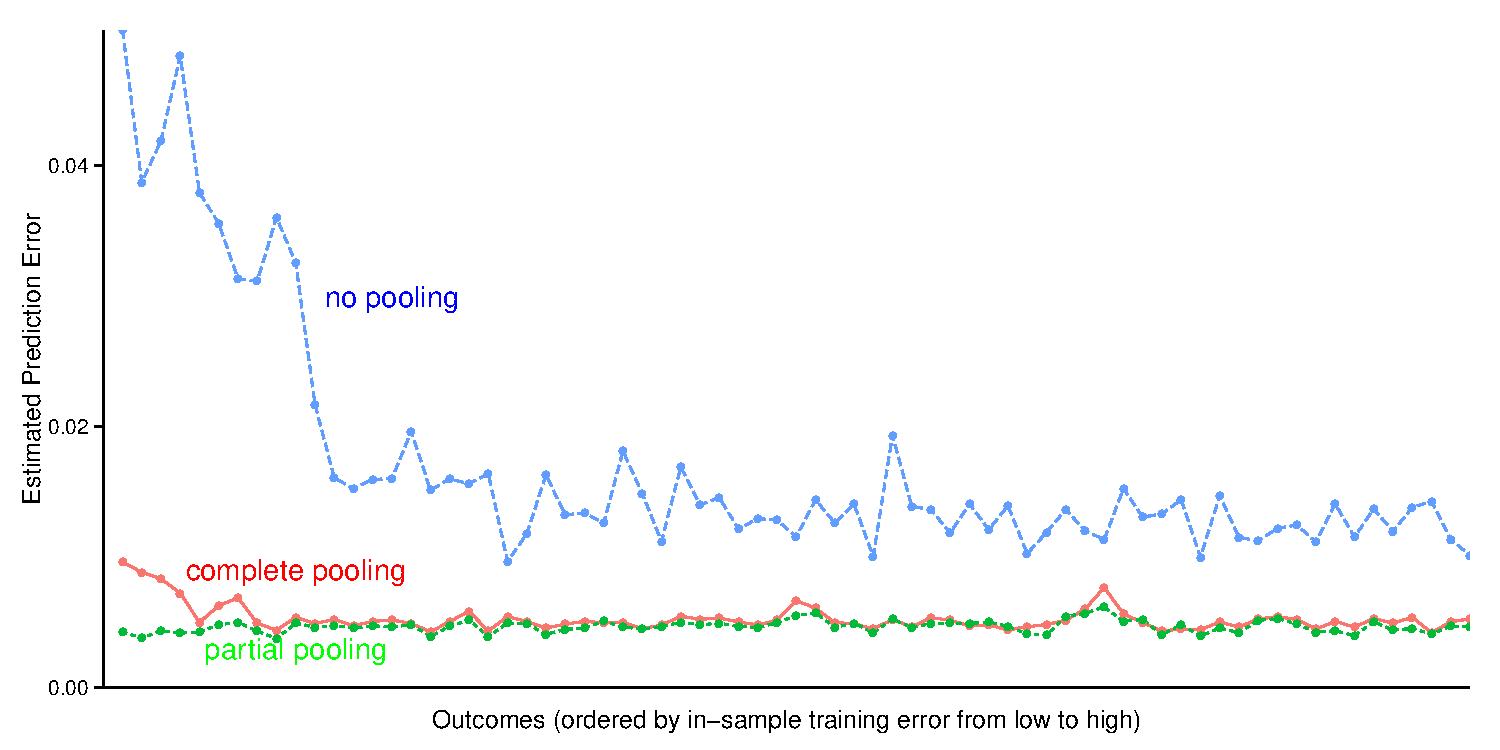
\includegraphics[width=\textwidth]{alloutcomesx1.pdf}
  \caption{\em Measure of fit (estimated prediction error) for all response outcomes
    in the 2006 Cooperative Congressional Election Survey. Outcomes are ordered by the lower bound
    (in-sample loss of the saturated model). The no pooling model
    gives a bad fit.  Partial pooling does best but in most cases is almost indistinguishable from complete pooling under the cross-validation criterion.}
  \label{fig:figx1}
\end{figure*}

I begin by estimating the prediction errors of all outcomes in the
survey. The results are shown in Figure\textasciitilde{}\ref{fig:figx1}.
The \(x\)-axis is ordered by the in-sample training loss of the
saturated model \(TL(M_{\text{s}},D)\), which I use as a surrogate for a
lower bound of predictive loss. For complete pooling and partial
pooling, the prediction error stays stable across different outcomes,
while the no pooling model has huge prediction error for outcomes with
small lower bounds. This finding makes sense since these are the
settings where overfitting is most severe (saturated models achieve the
lowest in-sample training error). However, the difference in prediction
error between complete pooling and partial pooling seems negligible.
Partial pooling is giving essentially the same result as complete
pooling, at least according to cross-validation on individual survey
responses.

\begin{figure*}[p!]
  \centering
  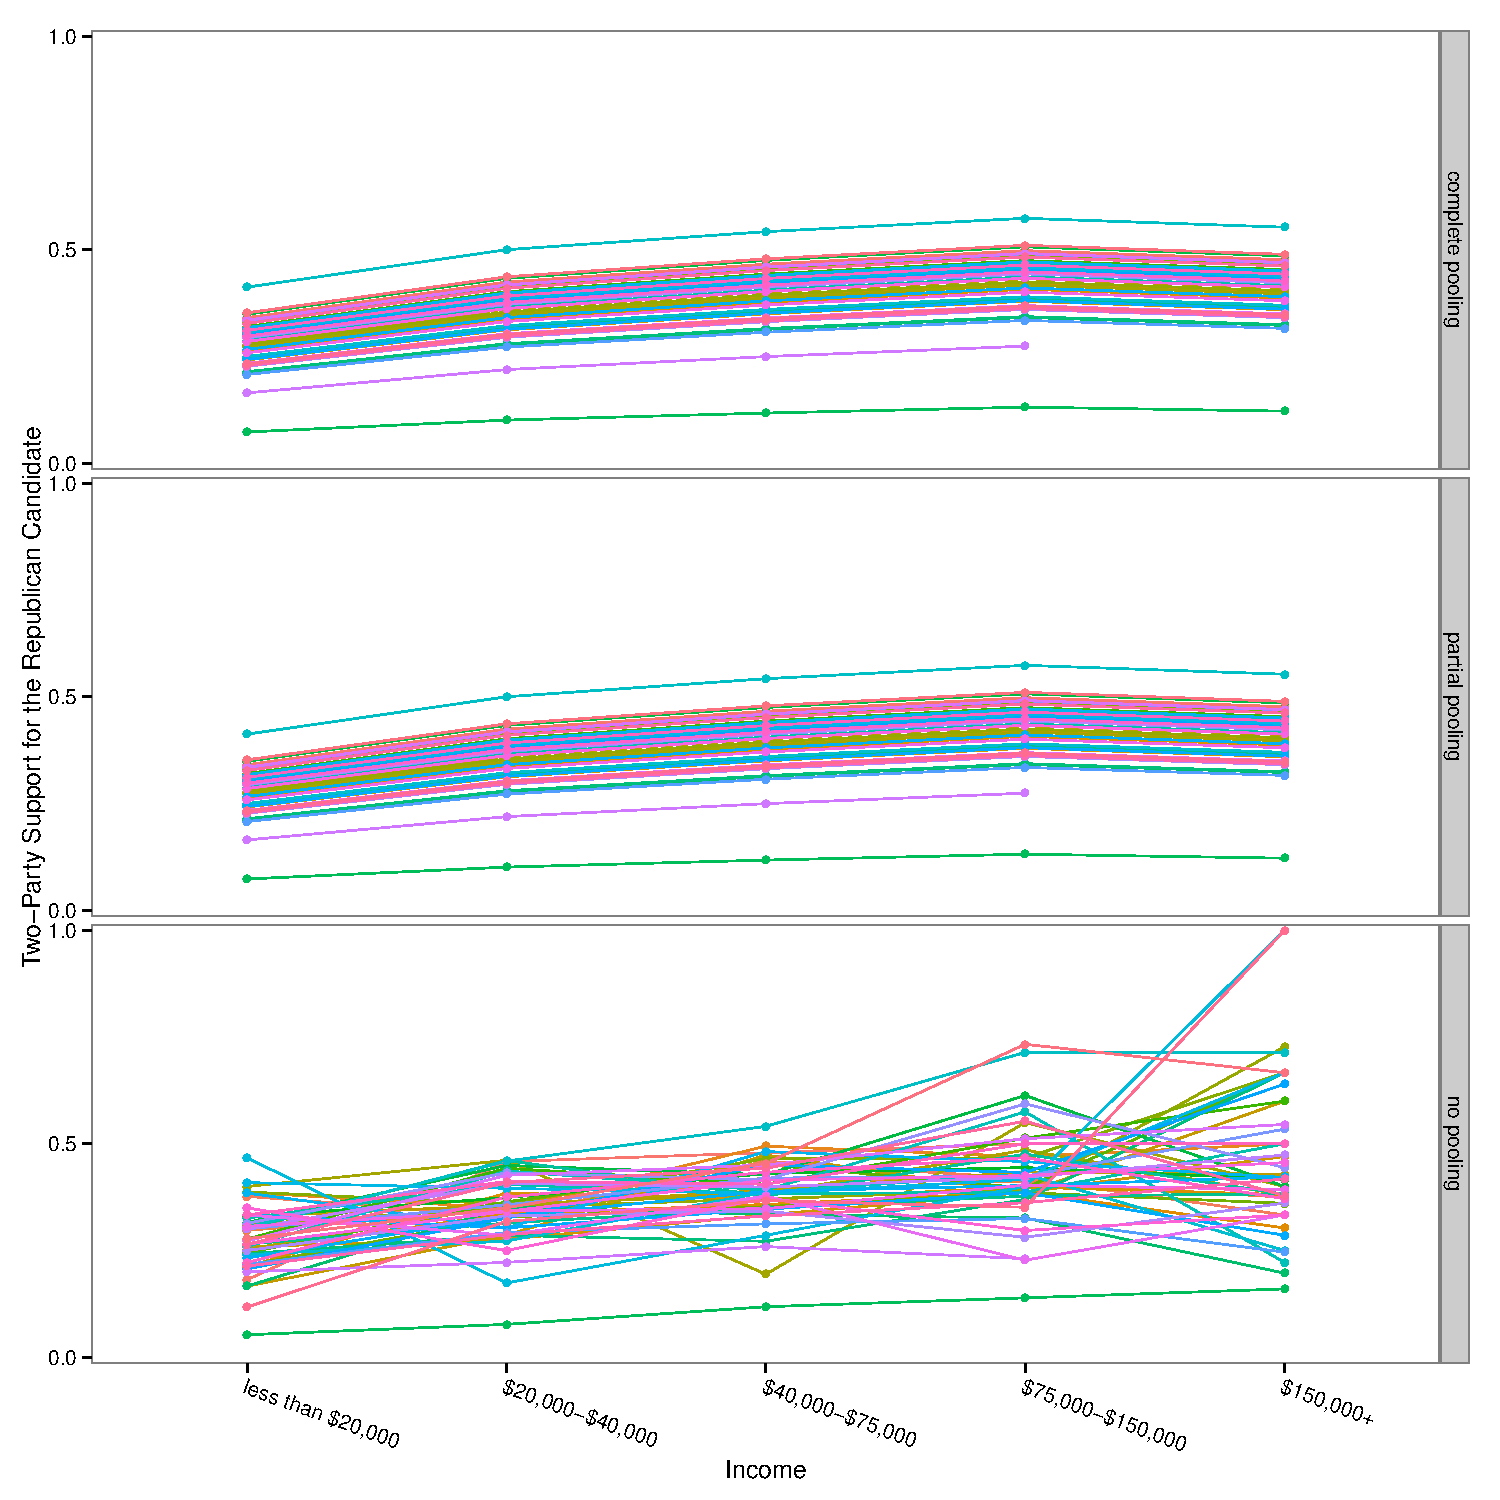
\includegraphics[width=.5\textwidth]{esti_all_bglmer}
  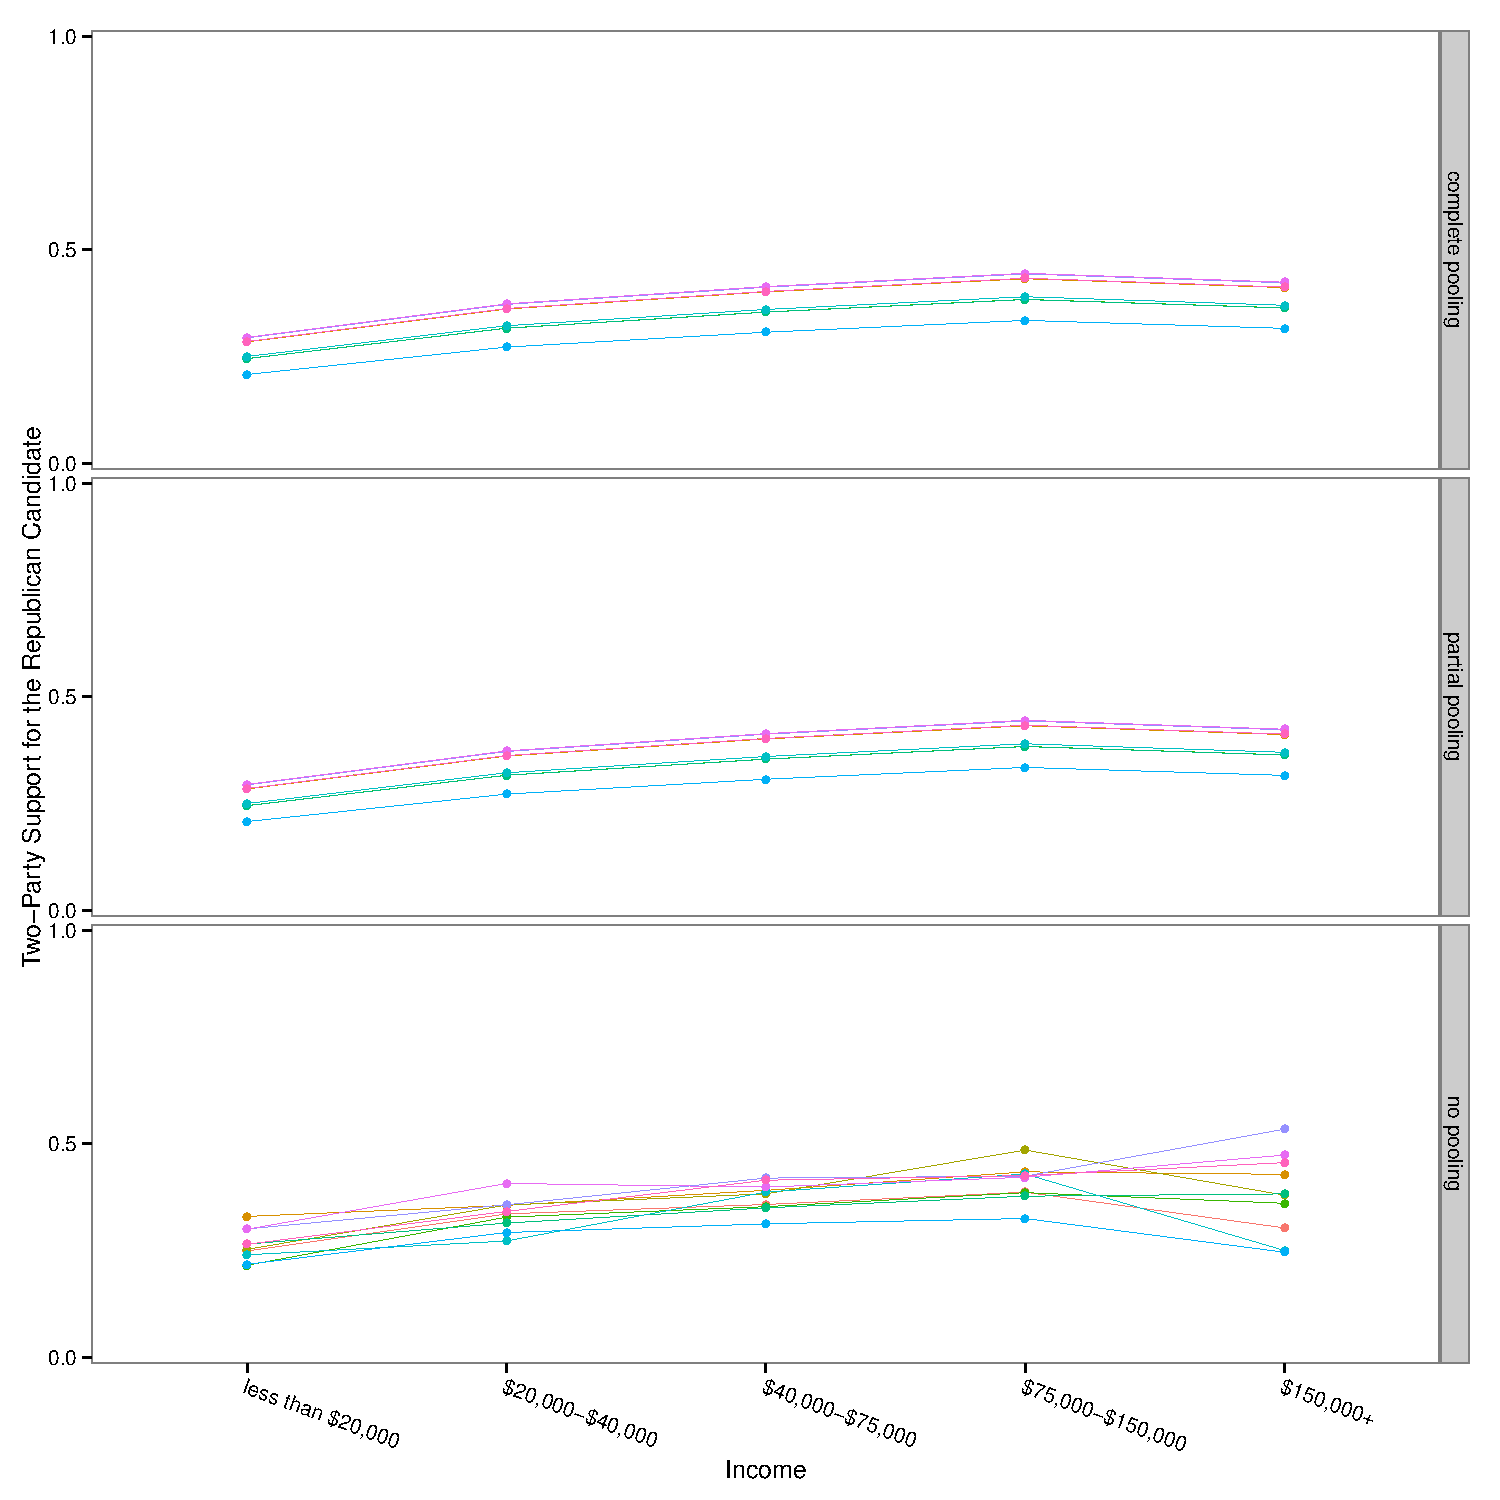
\includegraphics[width=.5\textwidth]{esti_big_bglmer}
  \caption{\em Left panel: Cell proportion estimates for three models of vote
    intention. Each line is a state. The
    partial pooling model pools so much that it is indistinguishable from
    complete pooling. Right panel: The same estimates for the 10 most populous
    states. Still, partial pooling estimates are similar to complete pooling
    estimates.}
  \label{fig:234}
\end{figure*}

This seems to suggest that partial pooling does not have enough
information to estimate cell-to-cell variation, thus giving an overly
conservative estimate. Indeed, when I plot the estimates of
\(\pi_{j_1j_2}\) for one particular outcome, vote preference for in the
congressional election (see the left panel of
Figure\textasciitilde{}\ref{fig:234}), the estimates from partial
pooling are almost identical to those from complete pooling. Even for
populous states where, because of their large sample size, the amount of
partial pooling should be small, there are no major differences between
estimates from partial pooling model and estimates from complete pooling
model (see the right panel of Figure\textasciitilde{}\ref{fig:234}).
This pattern is consistent across different outcomes.

Although partial pooling is intrinsically better than complete
pooling, it seems that the given data are not sufficient for the partial
pooling model to pick up the interaction and unpool the estimates
appropriately. It is a result of the particular characteristics of this
data set? There are three factors determining the structure of the data
that might affect the extent of pooling of the model. First is the
sample size. If I increase the sample size to a sufficiently large
level, the partial pooling model will be able to partially pool the
estimates to an appropriate amount. As sample size grows, the no pooling
model will eventually have the same performance as partial pooling, and
it might be interesting to see at what point the saturated model becomes
acceptable. The second factor affecting the relative performance of the
different models is the size of the interactions that are being
estimated, and the third factor is the level of imbalance in the
hierarchical structure. Survey data classified by demographic and
geographic predictors are typically highly unbalanced due to the long
tails of sizes typical in taxonomic structures (Mandelbrot 1955). For
example, the 2006 CCES includes 3,637 respondents from California but
only 131 from Arkansas. This unbalanced structure will affect the amount
of pooling performed by a multilevel model.

In the following subsections, I conduct simulations that vary sample
size and the structure of the cells to investigate how these factors
affect the relative performance of the three models as captured by
cross-validation.

\subsection{How Sample Size Changes the
Dynamics}\label{how-sample-size-changes-the-dynamics}

\begin{figure}[p!]
  \centering
  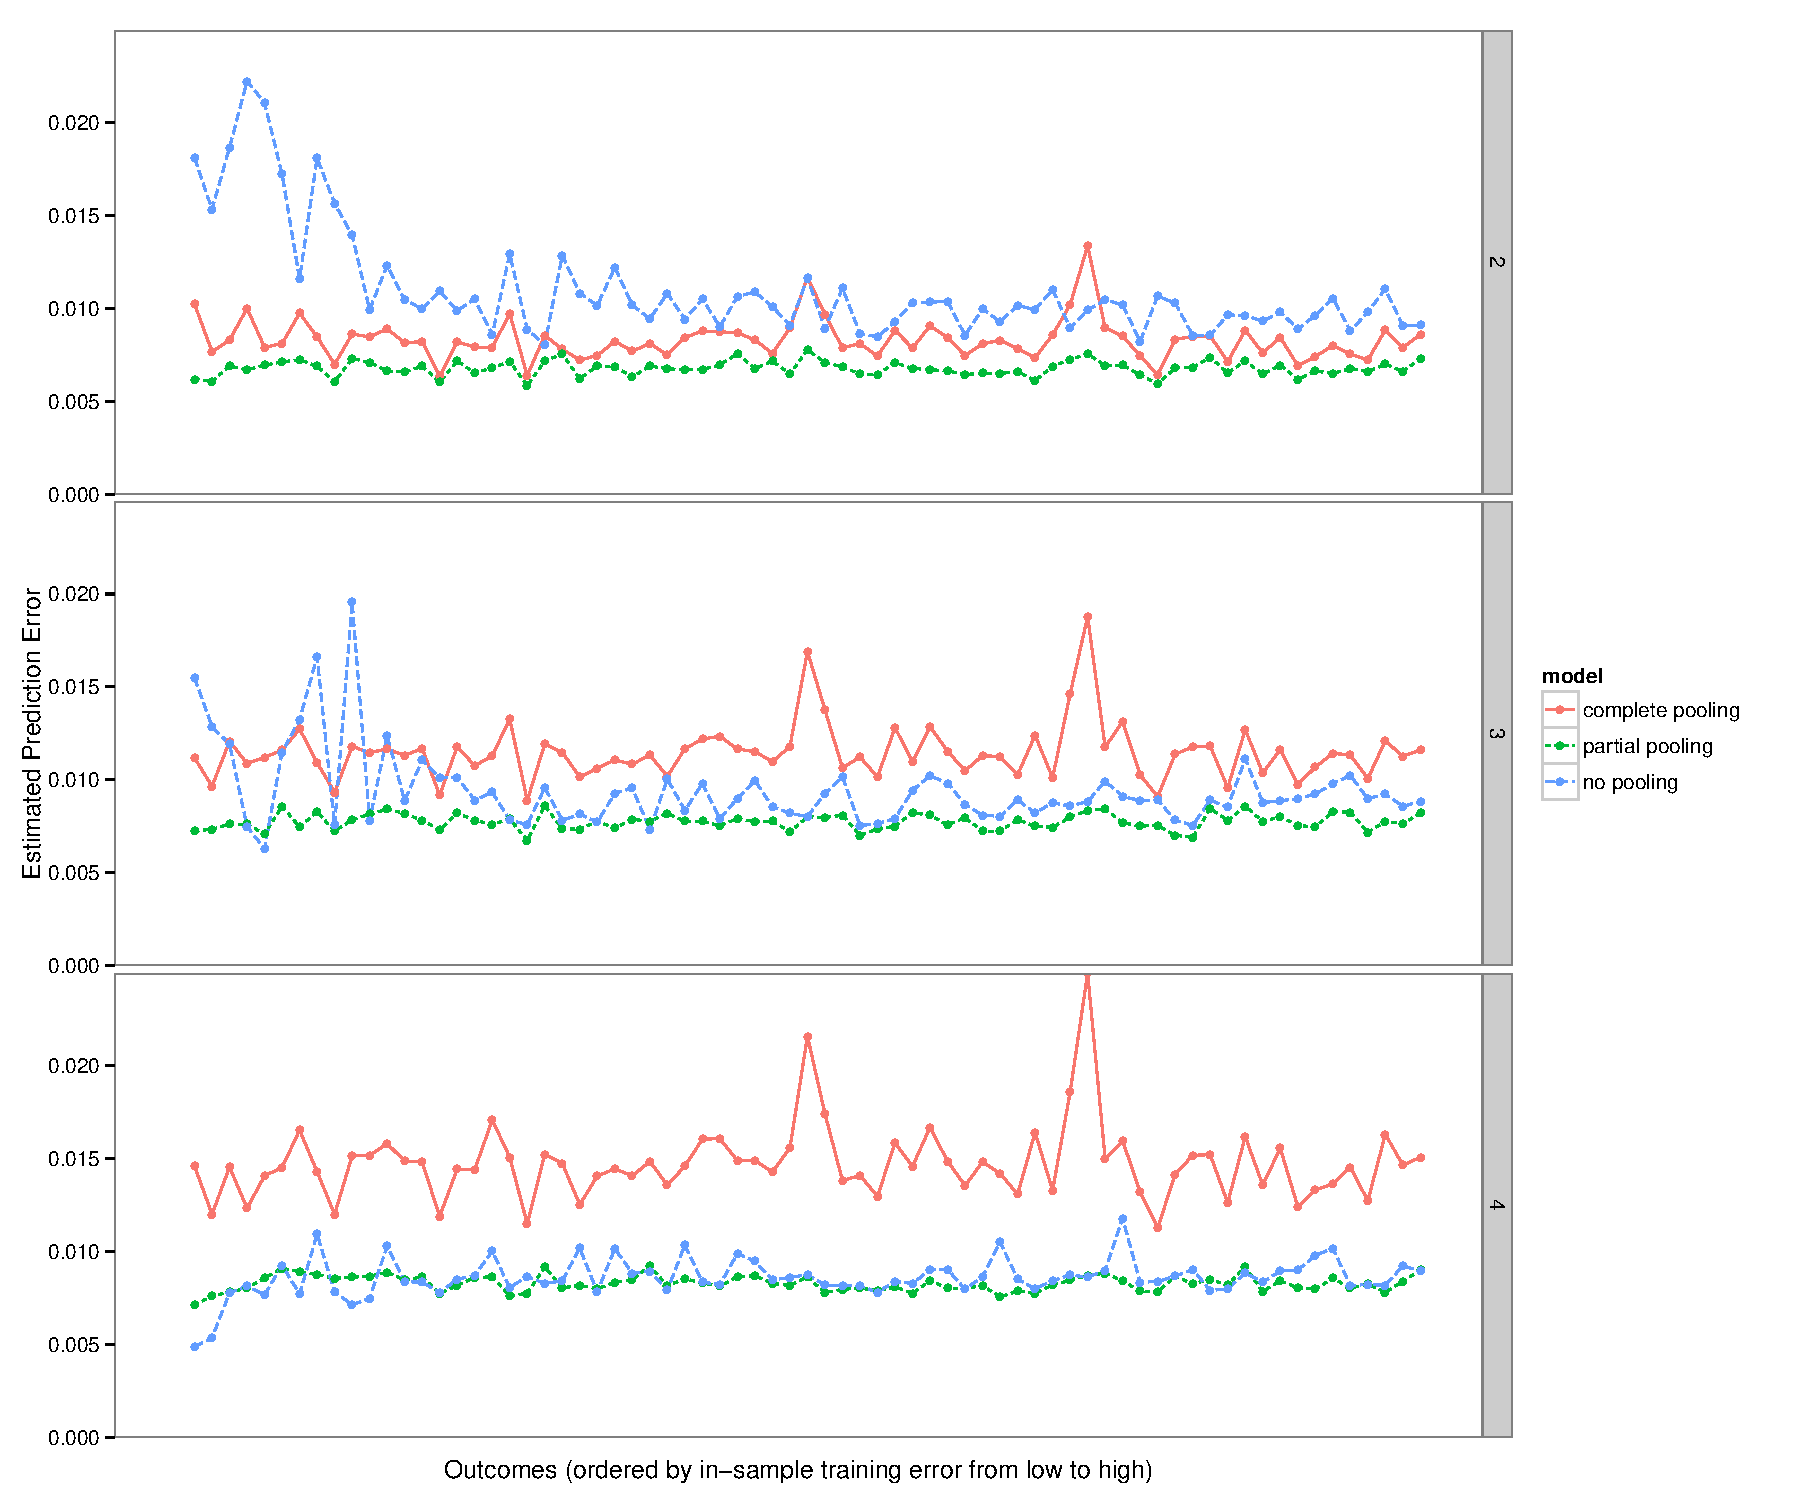
\includegraphics[width=\textwidth]{outcome234.pdf}
  \caption{\em Estimated prediction error of all response outcomes for augmented
    data sets. From top to bottom, the data sets have 2, 3, and 4 times as many
    data points as the original data set. The outcomes are ordered by the
    in-sample predictive loss. As sample size grows, complete pooling
    gradually gets worse and no pooling gets better.}
  \label{fig:figx234}
  \end{figure}

I artificially augment the data set by combining the data set with
itself. New data sets with sample size that are 2, 3 and 4 times as
large are generated. This augmentation still maintains the same level of
interactions and cell structure as those of the original data. Then I
estimate the prediction errors for all outcomes for the three models.
Results are plotted in Figure\textasciitilde{}\ref{fig:figx234}. As I
expected, as sample size grows, the prediction error of complete pooling
model, which is essentially a wrong model, dominates the other two;
while the prediction error of no pooling model keeps decreasing. When
the sample size is 4 times as large as the original data set, no pooling
model has almost the same prediction error as partial pooling model.
This makes sense, since the problem of overfitting eventual goes away if
there are sufficiently large sample size and fixed model structure.

\begin{figure*}[p!]
  \centering
  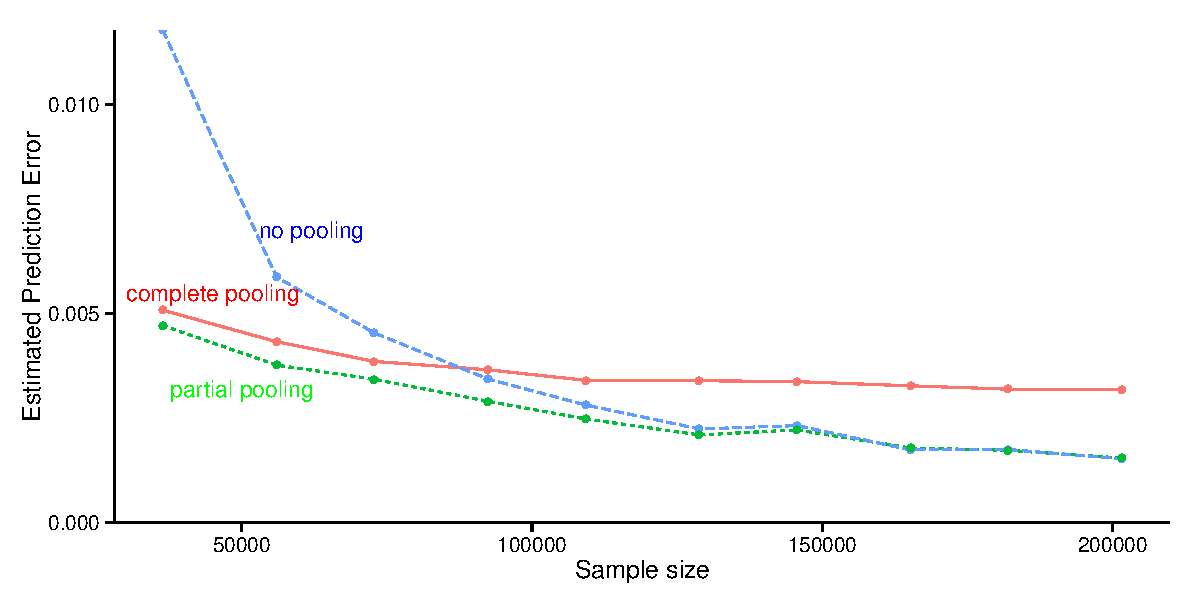
\includegraphics[width=\textwidth]{hourvote.pdf}
  \caption{\em Prediction error of the three models as sample size grows. The
    outcome under consideration is partisan vote preference in the upcoming
    congressional election. By this criterion, partial pooling and complete
    pooling perform similarly until sample size exceeds 50,000.}
  \label{fig:hourvote}
\end{figure*}

These results suggest that for a fixed data structure, partial pooling
decisively outperforms no pooling and complete pooling only for a
certain window of sample sizes. To have a closer look at the range of
the window, I look at one particular outcome, the vote preference in the
upcoming election for the U.S. House of Representatives. I augment the
sample size and plot the relative performance of the three models in
Figure\textasciitilde{}\ref{fig:hourvote}. Partial pooling model is
noticeably better than complete pooling in this setup when the total
sample size exceeds larger than 50,000. Other outcomes have similar
patterns.

\subsection{Balancedness of the Hierarchical
Structure}\label{balancedness-of-the-hierarchical-structure}

One possible explanation for the steep learning curve of the partial
pooling model is the highly unbalanced structure of the data. Although
there are 50 states, the estimate of the covariance of the state random
effects might not be reliable since some of the states have small sample
sizes. To see how the balancedness of the structure affects the model, I
simulate a data set based on partial pooling estimates from the original
data set, but make each demographic-geographic cells of roughly the same
size. The overall sample size is the same as that of the real data.
Relative performance of the three models for all outcomes is plotted in
Figure\textasciitilde{}\ref{fig:figbal}. The graph shows that with
balanced hierarchical structure, at the same sample size and amount of
interaction, partial pooling kicks in much more quickly. Thus partial
pooling is consistently better than complete pooling in this scenario.
As in the previous analysis, I also look at the relative performance of
the three models as sample size grows. The results are plotted in
Figure\textasciitilde{}\ref{fig:hourvote_bal}.

\begin{figure}[p!]
  \centering
  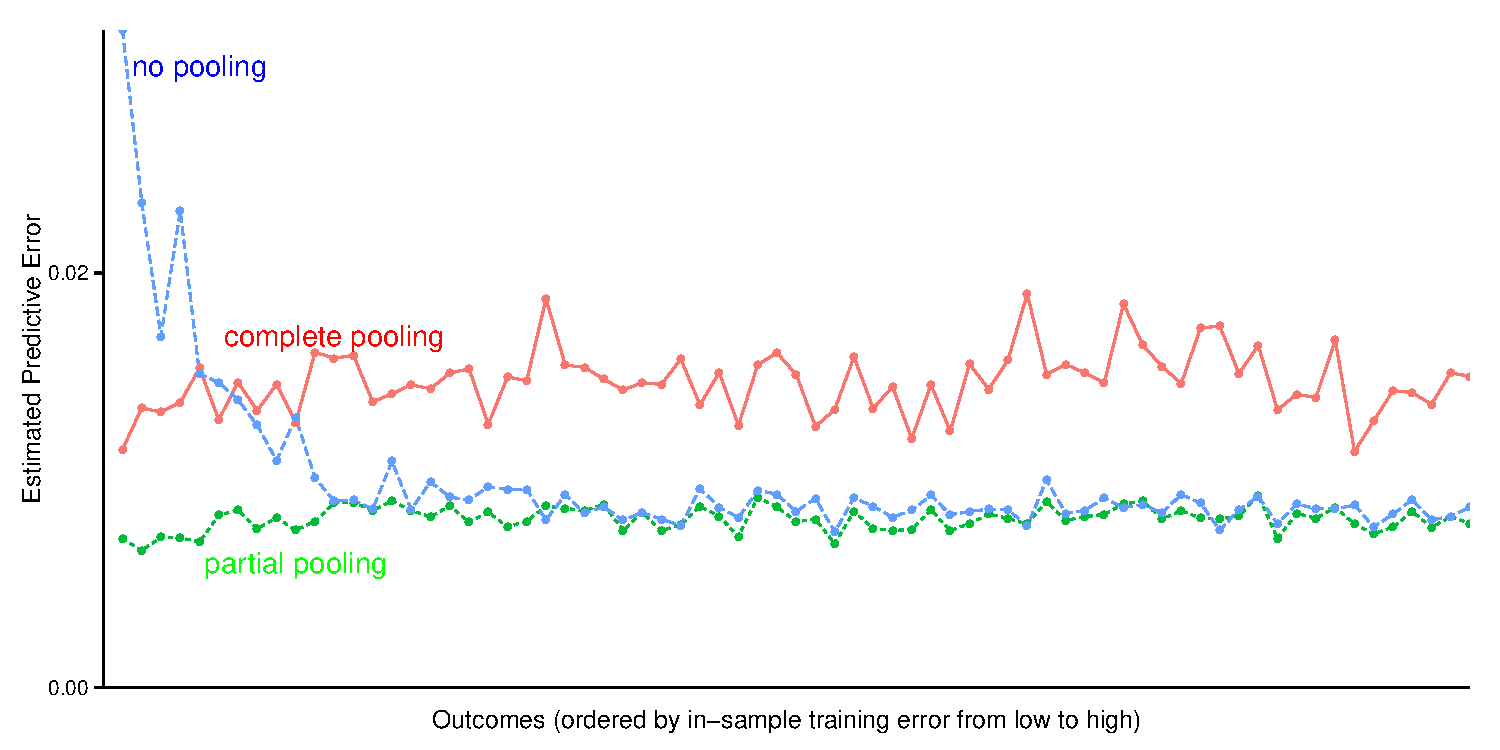
\includegraphics[width=\textwidth]{alloutcomesxbal.pdf}
  \caption{\em Measure of fit (prediction error) for all outcomes, ordered by
    in-sample training loss. The data set is simulated from real data set, and
    has the same sample size in total as the real data set, but keeping all
    demographic-geographic cells balanced. In this case, complete pooling model
    has much higher prediction errors than no pooling and partial
    pooling. Partial pooling is slightly but consistently better than no
    pooling. In particular, no pooling model has huge prediction error for
    outcomes that have smaller in-sample training loss.}
  \label{fig:figbal}
\end{figure}

\begin{figure}[p!]
  \centering
  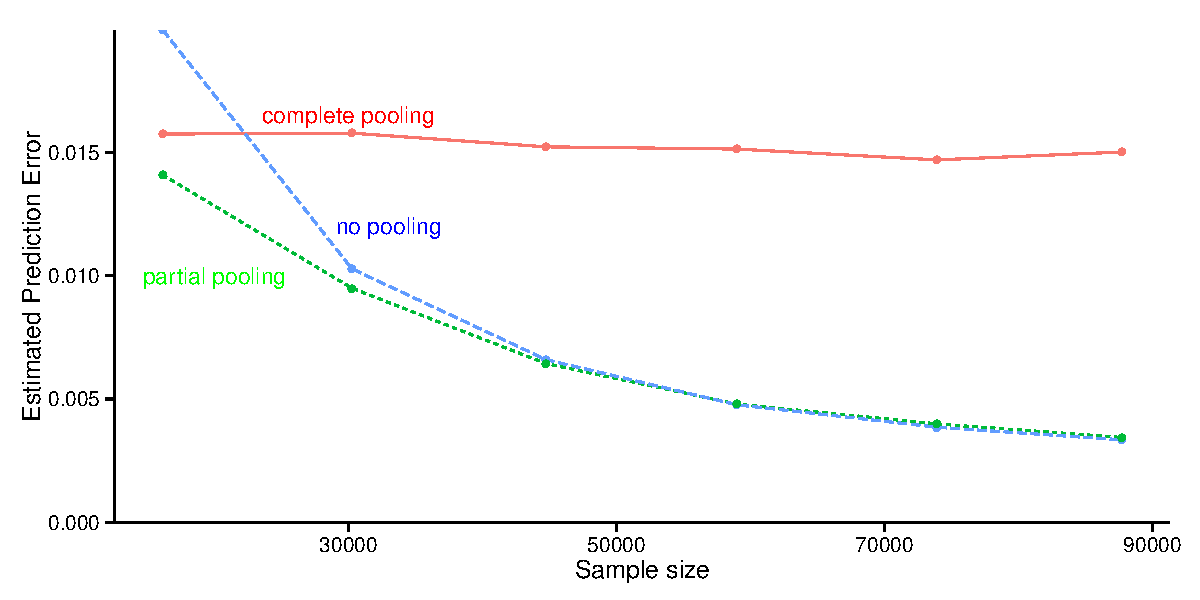
\includegraphics[width=\textwidth]{hourvote_bal.pdf}
  \caption{\em Prediction error of the three models as sample size grows under the
    simulated balanced data set. The outcome under consideration is the vote for
    the Republican candidate in the U.S House of Representatives. Partial
    pooling has the lowest prediction error when sample size is under 70,000.}
  \label{fig:hourvote_bal}
\end{figure}

\section{Discussion}\label{discussion}

Cross-validation is an important tool used to evaluate a wide variety of
statistical methods and has been widely used in model comparison when
predictive power is of concern. Some theoretical treatments have pointed
out situations where cross-validation might have problems. For example,
(Shao 1993) shows that, under the frequentist setting, using
leave-one-out cross-validation for linear model variable selection is
not consistent. However, the simplicity and transparency of
cross-validation gives it a near-universal appeal. In this paper, I
investigate the sensitivity of cross-validation as a model comparison
instrument in a cross-tabulated multilevel survey data set.

I set up the model selection problem, considering three models for these
structured data: the classical models of complete pooling and no
pooling, and a Bayesian multilevel model. The multilevel model captures
important interactions that are not included in the complete pooling
model, while at the same time avoiding the inevitable overfitting from
the no pooling model. However, the improvement of the multilevel model
as given by cross-validation is surprisingly tiny, almost negligible to
unsuspecting eyes. The problem is that improved fits with binary data
yield minuscule improvements in log loss, in moderate sample sizes
nearly indistinguishable from noise even if the improved estimates are
substantively important when aggregated (for example, state-level public
opinion). Simulations based on real data show that sample size and
structure of the cross-tabulated cells play important roles in the
relative margins of different models in cross-validation based model
selection. Caution should be exercised in applying prediction error for
model selection with structured data.

\newpage

\hyperdef{}{references}{\label{references}}
\section*{Bibliography}\label{bibliography}
\addcontentsline{toc}{section}{Bibliography}

\hyperdef{}{ref-lme4}{\label{ref-lme4}}
Bates, Douglas, Martin Maechler, and Ben Bolker. 2013. \emph{Lme4:
Linear mixed-effects models using s4 classes}.
\url{http://CRAN.R-project.org/package=lme4}.

\hyperdef{}{ref-burman1989comparative}{\label{ref-burman1989comparative}}
Burman, Prabir. 1989. ``A comparative study of ordinary
cross-validation, v-fold cross-validation and the repeated
learning-testing methods.'' \emph{Biometrika} 76(3): 503--514.

\hyperdef{}{ref-burman1994cross}{\label{ref-burman1994cross}}
Burman, Prabir, Edmond Chow, and Deborah Nolan. 1994. ``A
cross-validatory method for dependent data.'' \emph{Biometrika} 81(2):
351--358.

\hyperdef{}{ref-butticeux5f2013}{\label{ref-butticeux5f2013}}
Buttice, Matthew K., and Benjamin Highton. 2013. ``How does multilevel
regression and poststratification perform with conventional national
surveys?'' \emph{Political Analysis} 21(4): 449--467.

\hyperdef{}{ref-chung2013nondegenerate}{\label{ref-chung2013nondegenerate}}
Chung, Yeojin et al. 2013. ``A nondegenerate penalized likelihood
estimator for variance parameters in multilevel models.''
\emph{Psychometrika} 78(4): 685--709.

\hyperdef{}{ref-craven1978smoothing}{\label{ref-craven1978smoothing}}
Craven, Peter, and Grace Wahba. 1978. ``Smoothing noisy data with spline
functions.'' \emph{Numerische Mathematik} 31(4): 377--403.

\hyperdef{}{ref-blme}{\label{ref-blme}}
Dorie, Vincent. 2013. \emph{Blme: Bayesian linear mixed-effects models}.
\url{http://CRAN.R-project.org/package=blme}.

\hyperdef{}{ref-FayHerriot:1979}{\label{ref-FayHerriot:1979}}
Fay, R. E., and R. A. Herriot. 1979. ``Estimates of income for small
places: An application of james-stein procedures to census data.''
\emph{Journal of the American Statistical Association} 74: 269--277.

\hyperdef{}{ref-gelman2007data}{\label{ref-gelman2007data}}
Gelman, Andrew, and Jennifer Hill. 2007. \emph{Data analysis using
regression and multilevel/Hierarchical models}. Cambridge University
Press.

\hyperdef{}{ref-redstate}{\label{ref-redstate}}
Gelman, Andrew et al. 2009. \emph{Red state, blue state, rich state,
poor state: Why americans vote the way they do, second edition}.
Princeton University Press.

\hyperdef{}{ref-ghitzaux5f2013}{\label{ref-ghitzaux5f2013}}
Ghitza, Yair, and Andrew Gelman. 2013. ``Deep interactions with MRP:
Election turnout and voting patterns among small electoral subgroups.''
\emph{American Journal of Political Science} 57(3): 762--776.

\hyperdef{}{ref-groves2004survey}{\label{ref-groves2004survey}}
Groves, Robert M. 2004. 536 \emph{Survey errors and survey costs}. John
Wiley \& Sons.

\hyperdef{}{ref-hjort2010bayesian}{\label{ref-hjort2010bayesian}}
Hjort, Nils Lid. 2010. \emph{Bayesian nonparametrics}. Cambridge
University Press.

\hyperdef{}{ref-kale2011cross}{\label{ref-kale2011cross}}
Kale, Satyen, Ravi Kumar, and Sergei Vassilvitskii. 2011.
``Cross-validation and mean-square stability.'' In \emph{Innovations in
computer science,} Tsinghua University Press, p. 487--495.

\hyperdef{}{ref-laxux5f2009}{\label{ref-laxux5f2009}}
Lax, Jeffrey R., and Justin H. Phillips. 2009. ``How should we estimate
public opinion in the states?'' \emph{American Journal of Political
Science} 53(1): 107--121.

\hyperdef{}{ref-laxux5f2013}{\label{ref-laxux5f2013}}
Lax, Jeffrey R., and Justin H. Phillips. 2013. ``How should we estimate
sub-national opinion using MRP? Preliminary findings and
recommendations.'' \emph{Presented at Midwest Political Science
Association}.

\hyperdef{}{ref-Mandelbrot:1955}{\label{ref-Mandelbrot:1955}}
Mandelbrot, B. 1955. ``On the language of taxonomy: An outline of a
`thermostatistical' theory of systems of categories with willis
(natural) structure.'' In \emph{Information theory---Third london
symposium}, ed. Colin Cherry., p. 135--145.

\hyperdef{}{ref-pan2010survey}{\label{ref-pan2010survey}}
Pan, Sinno Jialin, and Qiang Yang. 2010. ``A survey on transfer
learning.'' \emph{IEEE Transactions on Knowledge and Data Engineering}
22(10): 1345--1359.

\hyperdef{}{ref-PriceGelmanNero1996}{\label{ref-PriceGelmanNero1996}}
Price, Phillip N., Anthony V. Nero, and Andrew Gelman. 1996. ``Bayesian
prediction of mean indoor radon concentrations for minnesota counties.''
\emph{Health Physics} 71: 922--936.

\hyperdef{}{ref-ruppert2003semiparametric}{\label{ref-ruppert2003semiparametric}}
Ruppert, David, Matt P Wand, and Raymond J Carroll. 2003.
\emph{Semiparametric regression}. Cambridge University Press.

\hyperdef{}{ref-seeger2008cross}{\label{ref-seeger2008cross}}
Seeger, Matthias W. 2008. ``Cross-validation optimization for large
scale structured classification kernel methods.'' \emph{Journal of
Machine Learning Research} 9: 1147--1178.

\hyperdef{}{ref-shao1993linear}{\label{ref-shao1993linear}}
Shao, Jun. 1993. ``Linear model selection by cross-validation.''
\emph{Journal of the American statistical Association} 88(422):
486--494.

\hyperdef{}{ref-Vehtari2012a}{\label{ref-Vehtari2012a}}
Vehtari, Aki, and Janne Ojanen. 2012. ``A survey of bayesian predictive
methods for model assessment, selection and comparison.''
\emph{Statistics Surveys} 6: 142--228.

\hyperdef{}{ref-wang2014difficulty}{\label{ref-wang2014difficulty}}
Wang, Wei, and Andrew Gelman. 2014. ``Difficulty of selecting among
multilevel models using predictive accuracy.'' \emph{Statistics and Its
Interface} 7: 1--8.

\hyperdef{}{ref-wang2014forecasting}{\label{ref-wang2014forecasting}}
Wang, Wei et al. 2014. ``Forecasting elections with non-representative
polls.'' \emph{International Journal of Forecasting}.


\part{Polling on Xbox}
\label{sec:xbox}
\chapter{Hierarchical Modeling of Non-Representative Polls}

In this chapter, I will discuss an application of hierarchical modeling
to non-representative survey sampling. As it is mentioned in the last
chapter, there is a dichotomy in modern survey research, the camp of
\emph{describers} and the camp of \emph{modelers}. However, at the heart
of modern opinion polling, for both \emph{describers} and
\emph{modelers}, is representative sampling, built around the goal that
every individual in a particular target population (e.g., registered or
likely U.S. voters) has the same probability of being sampled.
Non-representative sampling has fallen out of favor among pollsters as a
result of its inherent bias. I will show that, using an example of a
highly-biased poll on US presidential election conducted on Xbox gaming
platform, that hierarchical sampling can be used to remedy the bias and
help extract useful information from non-representative polls. This is a
joint work with David Rothschild, Sharad Goel, and Andrew Gelman, and
has been published in (Wang et al. 2014).

\section{A Brief History of Representative Sampling vs
Non-representative
Sampling}\label{a-brief-history-of-representative-sampling-vs-non-representative-sampling}

The wide-scale adoption of representative polling can largely be traced
to a pivotal polling mishap in the 1936 U.S. presidential election
campaign. During that campaign, the popular magazine \emph{Literary
Digest} conducted a mail-in survey that attracted over two million
responses, a huge sample even by modern standards. The magazine,
however, incorrectly predicted a landslide victory for Republican
candidate Alf Landon over the incumbent Franklin Roosevelt. Roosevelt,
in fact, decisively won the election, carrying every state except for
Maine and Vermont. As pollsters and academics have since pointed out,
the magazine's pool of respondents was highly biased: it consisted
mostly of auto and telephone owners as well as the magazine's own
subscribers, which underrepresented Roosevelt's core constituencies
(Squire 1988). During that same campaign, pioneering pollsters,
including George Gallup, Archibald Crossley, and Elmo Roper, used
considerably smaller but representative samples to predict the election
outcome with reasonable (Gosnell 1937). Accordingly, non-representative
or ``convenience sampling'' rapidly fell out of favor with polling
experts. Methods used for sampling have evolved over time, from
address-based, in-home interview sampling in the 1930s to random digit
dialing after the growth of landlines and cellphones; nevertheless,
leading polling organizations continue to put immense effort into
obtaining representative samples.

Two recent trends spur the interest for non-representative polls. First,
representative sampling is not nearly as representative as its name
suggests, and it is becoming less so. Random digit dialing (RDD), the
standard method in modern representative polling, has suffered
increasingly high non-response rates, both due to the general public's
growing reluctance to answer phone surveys, and expanding technical
means to screen unsolicited calls (Keeter et al. 2006). By one measure,
RDD response rates have decreased from 36\% in 1997 to 9\% in 2012
(Kohut et al. 2012). With such low response rates, even if the initial
pool of targets is representative, those who ultimately answer the phone
and elect to respond are almost certainly not, calling into question the
statistical benefits of such an approach. Related to dropping response
rates is a corresponding increase in cost, in both time and money, as
one needs to contact more and more potential respondents to find one
willing to participate. The second trend driving this research is that
with recent technological innovations, it is increasingly convenient and
cost-effective to collect large numbers of highly non-representative
samples via online surveys. What took several months for the
\emph{Literary Digest} editors to collect in 1936 can now take only a
few days and can cost just pennies per response. The challenge, of
course, is to extract meaningful signal from these unconventional
samples.

It is worth noting that the so-called ``Big Data'' is more often than
not a convenient sample, with potentially huge selection bias. Without
adequately addressing this issue first, any conclusion drawn from big
data analysis might be misleading.

\subsection{Xbox Data}\label{xbox-data}

The analysis is based on an opt-in poll continuously available on the
Xbox gaming platform during the 45 days preceding the 2012 U.S.
presidential election. Each day, three to five questions were posted,
one of which gauged voter intention with the standard query, ``If the
election were held today, who would you vote for?''. Respondents were
allowed to answer at most once per day. The first time they participated
in an Xbox poll, respondents were additionally asked to provide basic
demographic information about themselves, including their sex, race,
age, education, state, party ID, political ideology, and for whom they
voted in the 2008 presidential election. In total, 750,148 interviews
were conducted with 345,858 unique respondents---over 30,000 of whom
completed five or more polls---making this one of the largest ever
election panel studies.

\begin{figure}[p!]
  \centering
  \includegraphics[width=\textwidth]{"xbox_electorate_demo_comp"}
  \caption{A comparison of the demographic, partisan, and 2008 vote
    distribution in the Xbox dataset and the 2012 electorate (as
    measured by adjusted exit polls). The sex and age distributions, as one might expect, exhibit
  considerable differences.}
  \label{fig:demo_comp}
\end{figure}

\begin{figure}[p!]
  \centering
  \includegraphics[width=.8\textwidth]{"raw_response"}
  \caption{Daily (unadjusted) Xbox estimates of two-party Obama support during
    the 45 days leading up to the 2012 presidential election, which suggest a
    landslide victory for Mitt Romney. The dotted blue line indicates a
    consensus average of traditional polls (the daily aggregated polling results from Pollster.com), the horizontal dashed line at 52\%
    indicates the actual two-party vote share obtained by Barack Obama, and the
    vertical dotted lines give the dates of the three presidential debates.}
  \label{fig:raw_responses}
\end{figure}

Despite the large sample size, the pool of Xbox respondents is far from
representative of the voting population.
Figure\textasciitilde{}\ref{fig:demo_comp} compares the demographic
composition of the Xbox participants to that of the general electorate,
as estimated via the 2012 national exit poll. \footnote{For ease of
interpretation, in Figure~\ref{fig:demo_comp} states are grouped into 4 categories:
(1) battleground states (Colorado, Florida, Iowa, New Hampshire, Ohio, and
Virginia), the five states with the highest amounts of TV spending plus New
Hampshire, which had the highest per-capita spending; (2) quasi-battleground
states (Michigan, Minnesota, North Carolina, Nevada, New Mexico, Pennsylvania,
and Wisconsin), which round out the states where the campaigns and their
affiliates made major TV buys; (3) solid Obama states (California, Connecticut,
District of Columbia, Delaware, Hawaii, Illinois, Maine, Maryland,
Massachusetts, New Jersey, New York, Oregon, Rhode Island, Vermont, and
Washington); and (4) solid Romney states (Alabama, Alaska, Arizona, Arkansas,
Georgia, Idaho, Indiana, Kansas, Kentucky, Louisiana, Mississippi, Missouri,
Montana, Nebraska, North Dakota, Oklahoma, South Carolina, South Dakota,
Tennessee, Texas, Utah, West Virginia, and Wyoming).} The most striking
differences are for age and sex. As one might expect, young men dominate
the Xbox population: 18-to-29-year-olds comprise 65\% of the Xbox
dataset, compared to 19\% in the exit poll; and men make up 93\% of the
Xbox sample but only 47\% of the electorate. Political scientists have
long observed that both age and sex are strongly correlated with voting
preferences (Kaufmann and Petrocik 1999), and indeed these discrepancies
are apparent in the unadjusted time-series of Xbox voter intent shown in
Figure \ref{fig:raw_responses}. In contrast to estimates based on
traditional, representative polls (indicated by the dotted blue line in
Figure \ref{fig:raw_responses}), the uncorrected Xbox sample suggests a
landslide victory for Mitt Romney, reminiscent of the infamous
\emph{Literary Digest} error.

\section{Estimating voter intent with multilevel regression and
poststratification}\label{estimating-voter-intent-with-multilevel-regression-and-poststratification}

\subsection{Multilevel regression and
poststratification}\label{multilevel-regression-and-poststratification}

To transform the raw Xbox data into accurate estimates of voter intent
in the general electorate, I make use of the rich demographic
information that respondents provide. In particular I
\emph{poststratify} the raw Xbox responses to mimic a representative
sample of likely voters. Poststratification is a popular method for
correcting for known differences between sample and target populations
(Little 1993). The core idea is to partition the population into cells
(e.g., based on combinations of various demographic attributes), use the
sample to estimate the response variable within each cell, and finally
to aggregate the cell-level estimates up to a population-level estimate
by weighting each cell by its relative proportion in the population.
Using \(y\) to indicate the outcome of interest, the poststratification
estimate is defined by,

\begin{equation*}
\hat{y}^{\text{PS}}=\frac{\sum_{j=1}^JN_j\hat{y}_j}{\sum_{j=1}^JN_j}
\end{equation*}

\noindent where \(\hat{y}_j\) is the estimate of \(y\) in cell \(j\),
and \(N_j\) is the size of the \(j\)-th cell in the population. An
estimate of \(y\) can be analogously derived at any subpopulation level
\(s\) (e.g., voter intent in a particular state) by

\begin{equation*}
\hat{y}_s^{\text{PS}}=\frac{\sum_{j\in J_s}N_j\hat{y}_j}{\sum_{j\in J_s}N_j}
\end{equation*}

\noindent where \(J_s\) is the set of all cells that comprise \(s\). As
is readily apparent from the form of the poststratification estimator,
the key is to obtain accurate cell-level estimates, as well as estimates
for the cell sizes.

One of the most common ways to generate cell-level estimates is to
simply average sample responses within each cell. If it is assumed that
within a cell the sample is drawn at random from the larger population,
this yields an unbiased estimate. However, this assumption of cell-level
simple random sampling is only reasonable when the partition is
sufficiently fine; on the other hand, as the partition becomes finer,
the cells become sparse, and the empirical sample averages become
unstable. I address these issues by instead generating cell-level
estimates via a regularized regression model, namely multilevel
regression.

This combined model-based poststratification strategy, known as
multilevel regression and poststratification (MRP), has been used to
obtain accurate small-area subgroup estimates, such as for public
opinion and voter turnout in individual states and demographic subgroups
{[}Park, Gelman, and Bafumi (2004);Lax and Phillips (2009);Ghitza and
Gelman (2013)\}.

More formally, applying MRP in this setting comprises two steps. First a
Bayesian hierarchical model is fit to obtain estimates for sparse
poststratification cells; second, one averages over the cells, weighting
by a measure of forecasted voter turnout, to get state and
national-level estimates. Specifically, I generate the cells by
considering all possible combinations of sex (2 categories), race (4
categories), age (4 categories), education (4 categories), state (51
categories), party ID (3 categories), ideology (3 categories) and 2008
vote (3 categories), which partition the data into 176,256
cells.\footnote{All
demographic variables are collected prior to respondents' first poll,
alleviating concerns that respondents may adjust their demographic responses to
be inline with their voter intention (e.g., a new Obama supporter switching his
or her party ID from Republican to Democrat).} I fit two, nested
multilevel logistic regressions to estimate candidate support in each
cell. The first of the two models predicts whether a respondent supports
a major-party candidate (i.e., Obama or Romney), and the second predicts
support for Obama given that the respondent supports a major-party
candidate. Following the notation of (Gelman and Hill 2007), the first
model is given by

\begin{align}\label{eqn:m1}
  \text{Pr}(Y_i \in \, &\{\text{Obama, Romney}\})=\nonumber\\
  &\text{logit}^{-1}\big(\alpha_0+  \alpha_1\text{(state last vote share)} \\
  &+ a^{\text{state}}_{j[i]}+a^{\text{edu}}_{j[i]}+a^{\text{sex}}_{j[i]}+a^{\text{age}}_{j[i]}
  +a^{\text{race}}_{j[i]}+a^{\text{party ID}}_{j[i]}
  +b^{\text{ideology}}_{j[i]} + b^{\text{last vote}}_{j[i]} \big)\nonumber
\end{align}

where \(\alpha_0\) is the fixed baseline intercept, and \(\alpha_1\) is
the fixed slope for Obama's fraction of two-party vote share in the
respondent's state in the last presidential election. The terms
\(a^{\text{state}}_{j[i]}\), \(a^{\text{edu}}_{j[i]}\),
\(a^{\text{sex}}_{j[i]}\) and so on---which in general is denote by
\(a^{\text{var}}_{j[i]}\)---correspond to varying coefficients
associated with each categorical variable. Here the subscript \(j[i]\)
indicates the cell to which the \(i\)-th respondent belongs. For
example, \(a^{\text{age}}_{j[i]}\) takes values from
\(\{a^{\text{age}}_{18-29}, a^{\text{age}}_{30-44}, a^{\text{age}}_{45-64}, a^{\text{age}}_{65+}\}\)
depending on the cell membership of the \(i\)-th respondent. The varying
coefficients \(a_{j[i]}^{\text{var}}\) are given independent prior
distributions

\begin{equation*}
a^{\text{var}}_{j[i]}\sim N(0,\sigma^2_\text{var}).
\end{equation*}

\noindent To complete the full Bayesian specification, the variance
parameters are assigned a hyperprior distribution

\begin{equation*}\sigma^2_\text{var}\sim \text{inv-}\chi^2(\nu, \sigma_0^2),
\end{equation*}

\noindent with a weak prior specification for the remaining parameters,
\(\nu\) and \(\sigma_0\). The benefit of using a multilevel model is
that estimates for relatively sparse cells can be improved through
``borrowing strength'' from demographically similar cells that have
richer data. Similarly, the second model is defined by

\begin{align}  \label{eqn:m2}
  \text{Pr}(Y_i = \, &\text{Obama} \, |\, Y_i\in\{\text{Obama, Romney}\})=\nonumber\\
  &\text{logit}^{-1}\big(\beta_0+ \beta_1\text{(state last vote share)} \\
  & + b^{\text{state}}_{j[i]}+b^{\text{edu}}_{j[i]}+b^{\text{sex}}_{j[i]}+b^{\text{age}}_{j[i]}
  +b^{\text{race}}_{j[i]}+b^{\text{party ID}}_{j[i]} +
  b^{\text{ideology}}_{j[i]} + b^{\text{last vote}}_{j[i]}
 \big)\nonumber
\end{align}

\noindent and

\begin{align*}
  b^{\text{var}}_{j[i]}&\sim N(0,\eta^2_\text{var}),\\
  \eta^2_\text{var}&\sim \text{inv-}\chi^2(\mu, \eta_0^2).
  \end{align*}

Jointly, Eqs.\textasciitilde{}\eqref{eqn:m1} and \eqref{eqn:m2} define a
Bayesian model that describes the data. Ideally, a fully Bayesian
analysis would be performed to obtain the posterior distribution of the
parameters. However, for computational convenience, I use the
approximate marginal maximum likelihood estimates obtained from the
\texttt{glmer()} function in the \texttt{R} package \texttt{lme4}
(Bates, Maechler, and Bolker 2013).

Having detailed the multilevel regression step, I now turn to
poststratification, where cell-level estimates are weighted by the
proportion of the electorate in each cell and aggregated to the
appropriate level (e.g., state or national). To compute cell weights,
cross-tabulated population data is needed. One commonly used source for
such data is the Current Population Survey (CPS); however, the CPS does
not includes some key poststratification variables, such as party
identification. I thus instead use exit poll data from the 2008
presidential election. Exit polls are conducted on election day outside
voting stations to record the choices of exiting voters, and they are
generally used by researchers and news media to analyze the demographic
breakdown of the vote (after a post-election adjustment that aligns the
weighted responses to the reported state-by-state election results). In
total, 101,638 respondents were surveyed in the state and national exit
polls. I use the exit poll from 2008, not 2012, because this means that
in theory the method as described here could have been used to generate
real-time predictions during the 2012 election campaign. Admittedly,
this approach puts my prediction at a disadvantage since the demographic
shifts of the intervening four years cannot be captured. While combining
exit poll and CPS data would arguably yield improved results, for
simplicity and transparency I exclusively use the 2008 exit poll
summaries for poststratification.

\subsection{National and State Voter
Intent}\label{national-and-state-voter-intent}

Figure\textasciitilde{}\ref{fig:national_snap} shows the adjusted
two-party Obama support for the last 45 days of the election. \%The
daily voter intents for two-party Obama support at the national level
are \%illustrated in Figure \ref{fig:national_snap}. Compared with the
uncorrected estimates in Figure \ref{fig:raw_responses}, the
MRP-adjusted estimates yield a much more reasonable timeline of Obama's
standing over the course of the final weeks of the campaign. With a
clear advantage at the beginning, Obama's support slipped rapidly after
the first presidential debate---though never falling below 50\%---and
gradually recovered, building up a decisive lead in the final days.

On the day before the election, the estimate of voter intent is off by a
mere 0.6 percentage points from the actual outcome (indicated by the
dotted horizontal line). Voter intent in the weeks prior to the election
does not directly equate to an estimate of vote share on election
day---a point I return to in Section\textasciitilde{}\ref{sec:forecast}.
As such, it is difficult to evaluate the accuracy of the full
time-series of estimates. Nonetheless, I note that the estimates are not
only intuitively reasonable, but that they are also inline with
prevailing estimates based on traditional, representative polls. In
particular, the estimates roughly track---and are even arguably better
than---those from Pollster.com, one of the leading poll aggregators
during the 2012 campaign.

\begin{figure}[p!]
  \centering
  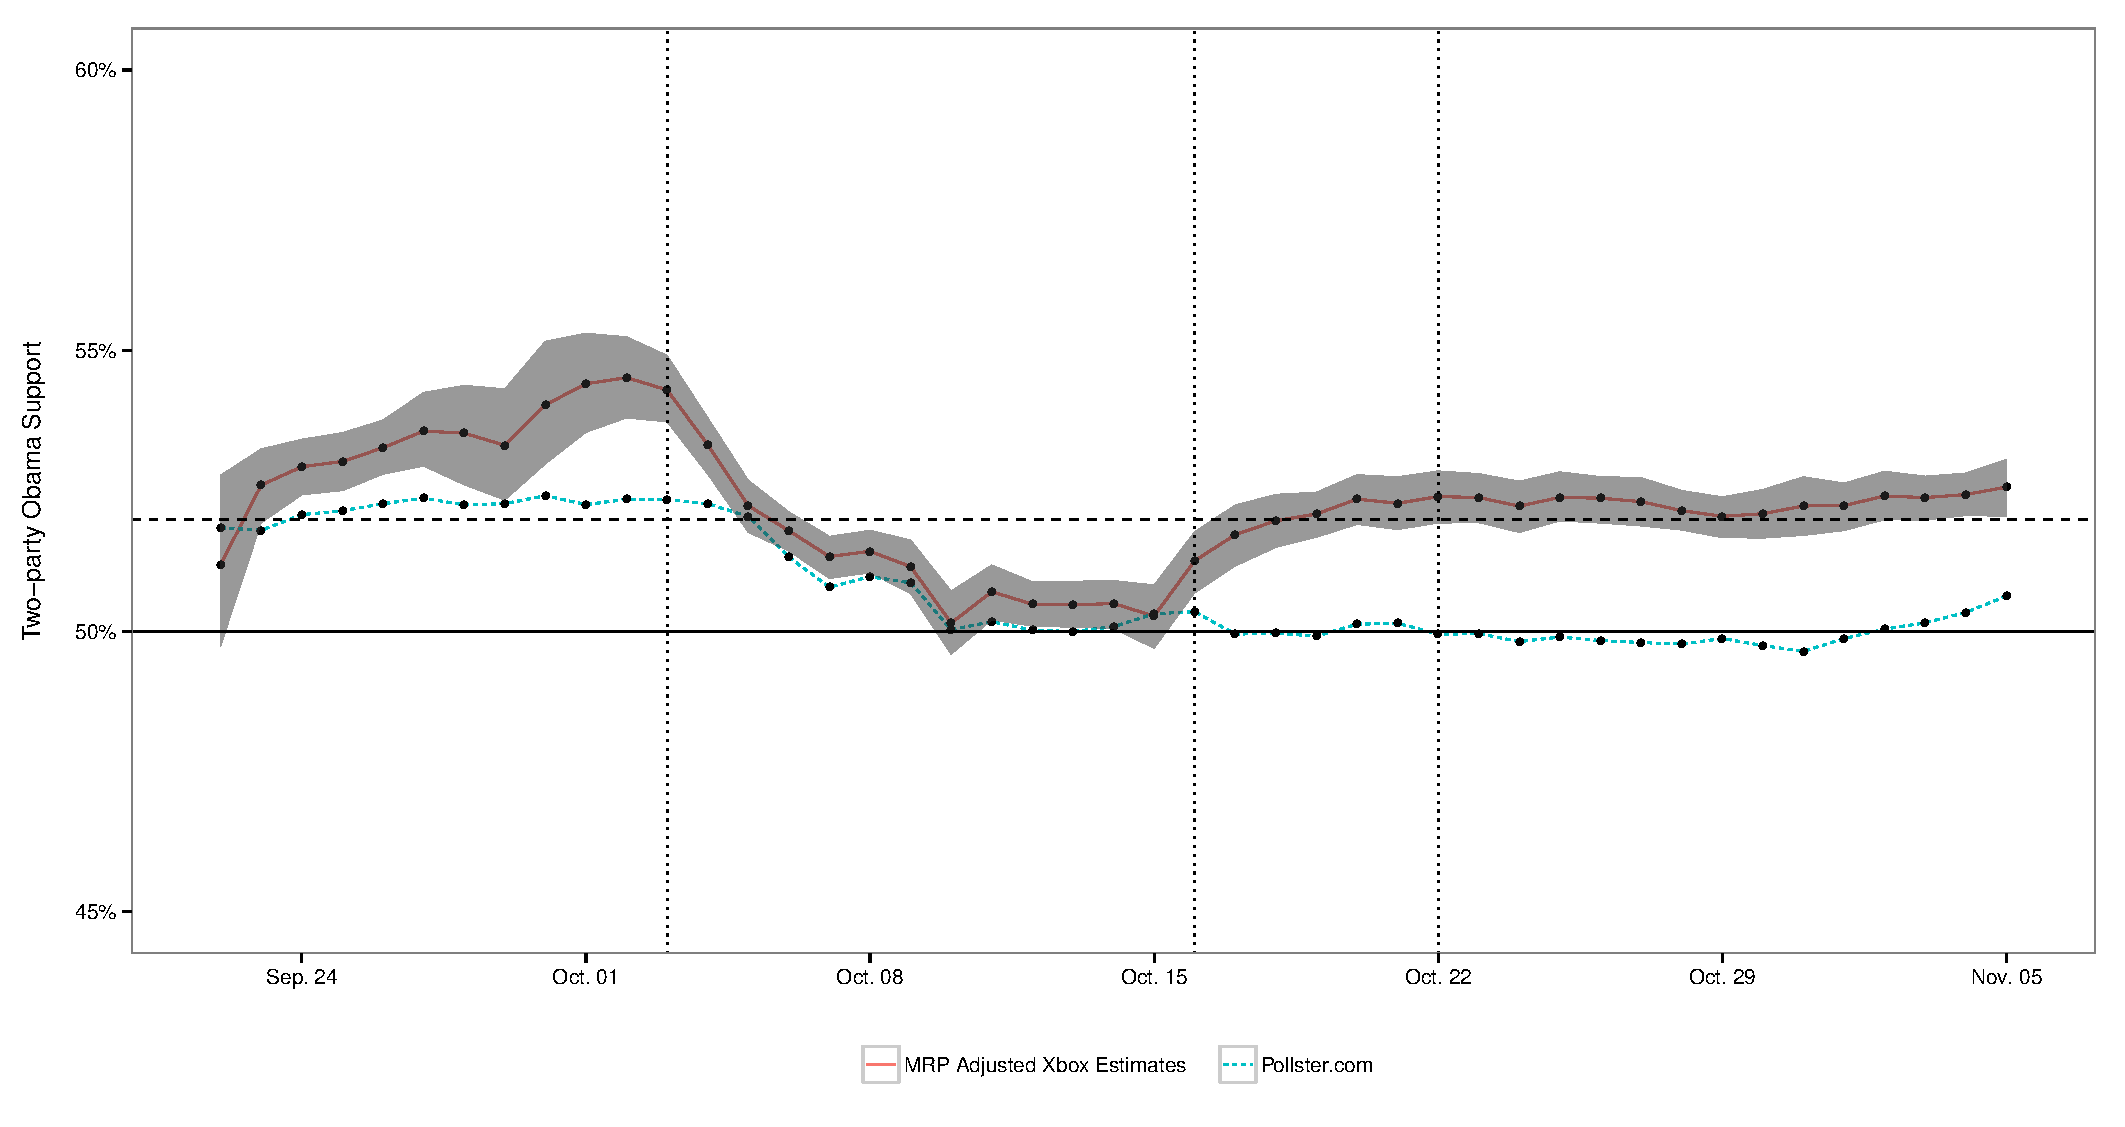
\includegraphics[width=.8\textwidth]{mrp_snapshots_national}
  \caption{National MRP-adjusted voter intent of two-party Obama support over
    the 45-day period and the associated 95\% confidence bands. The horizontal
    dashed line indicates the actual two-party Obama vote share. The three
    vertical dotted lines indicate the presidential debates. Compared with the raw
    responses in Figure \ref{fig:raw_responses}, the MRP-adjusted voter intent
    is much more reasonable, and voter intent in the last few days is very
    close to the actual outcome. For comparison, the daily aggregated polling
    results from Pollster.com, shown as the blue dotted line, are further away from the actual vote share
    than the estimates generated from the Xbox data in the last few days.}
  \label{fig:national_snap}
\end{figure}

National vote share receives considerable media attention, but
state-level estimates are particularly relevant for many stakeholders
given the role of the Electoral College in selecting the winner
(Rothschild 2013). forecast the joint probability of victory for each
candidate in Forecasting state-by-state races is a challenging problem
due to the interdependencies in state outcomes, \%and the joint
electoral votes has not yet become the standard forecast the logistical
difficulties of measuring state-level vote preference, and the effort
required to combine information from various sources (Lock and Gelman
2010). The MRP framework, however, provides a straightforward
methodology for generating state-level results. Namely, I use the same
cell-level estimates employed in the national estimate, as generated via
the multilevel model in Eqs.~\eqref{eqn:m1} and \eqref{eqn:m2}, and I
then poststratify to each state's demographic composition. In this
manner, the Xbox responses can be used to construct estimates of voter
intent over the last 45 days of the campaign for all 51 Electoral
College races.

Figure \ref{fig:state_snap} shows two-party Obama support for the 12
states with the most electoral votes. The state timelines share similar
trends (e.g., support for Obama dropping after the first debate), but
also have their own idiosyncratic movements, an indication of a
reasonable blend of national and state-level signals. To demonstrate the
accuracy of the MRP-adjusted estimates, I plot, in dotted blue lines in
Figure\textasciitilde{}\ref{fig:state_snap}, the estimates generated by
Pollster.com, which are broadly consistent with the state-level MRP
estimates. Moreover, across the 51 Electoral College races, the mean and
median absolute errors of the estimates on the day before the election
are just 2.5 and 1.8 percentage points, respectively.

\begin{figure}[p!]
  \centering
  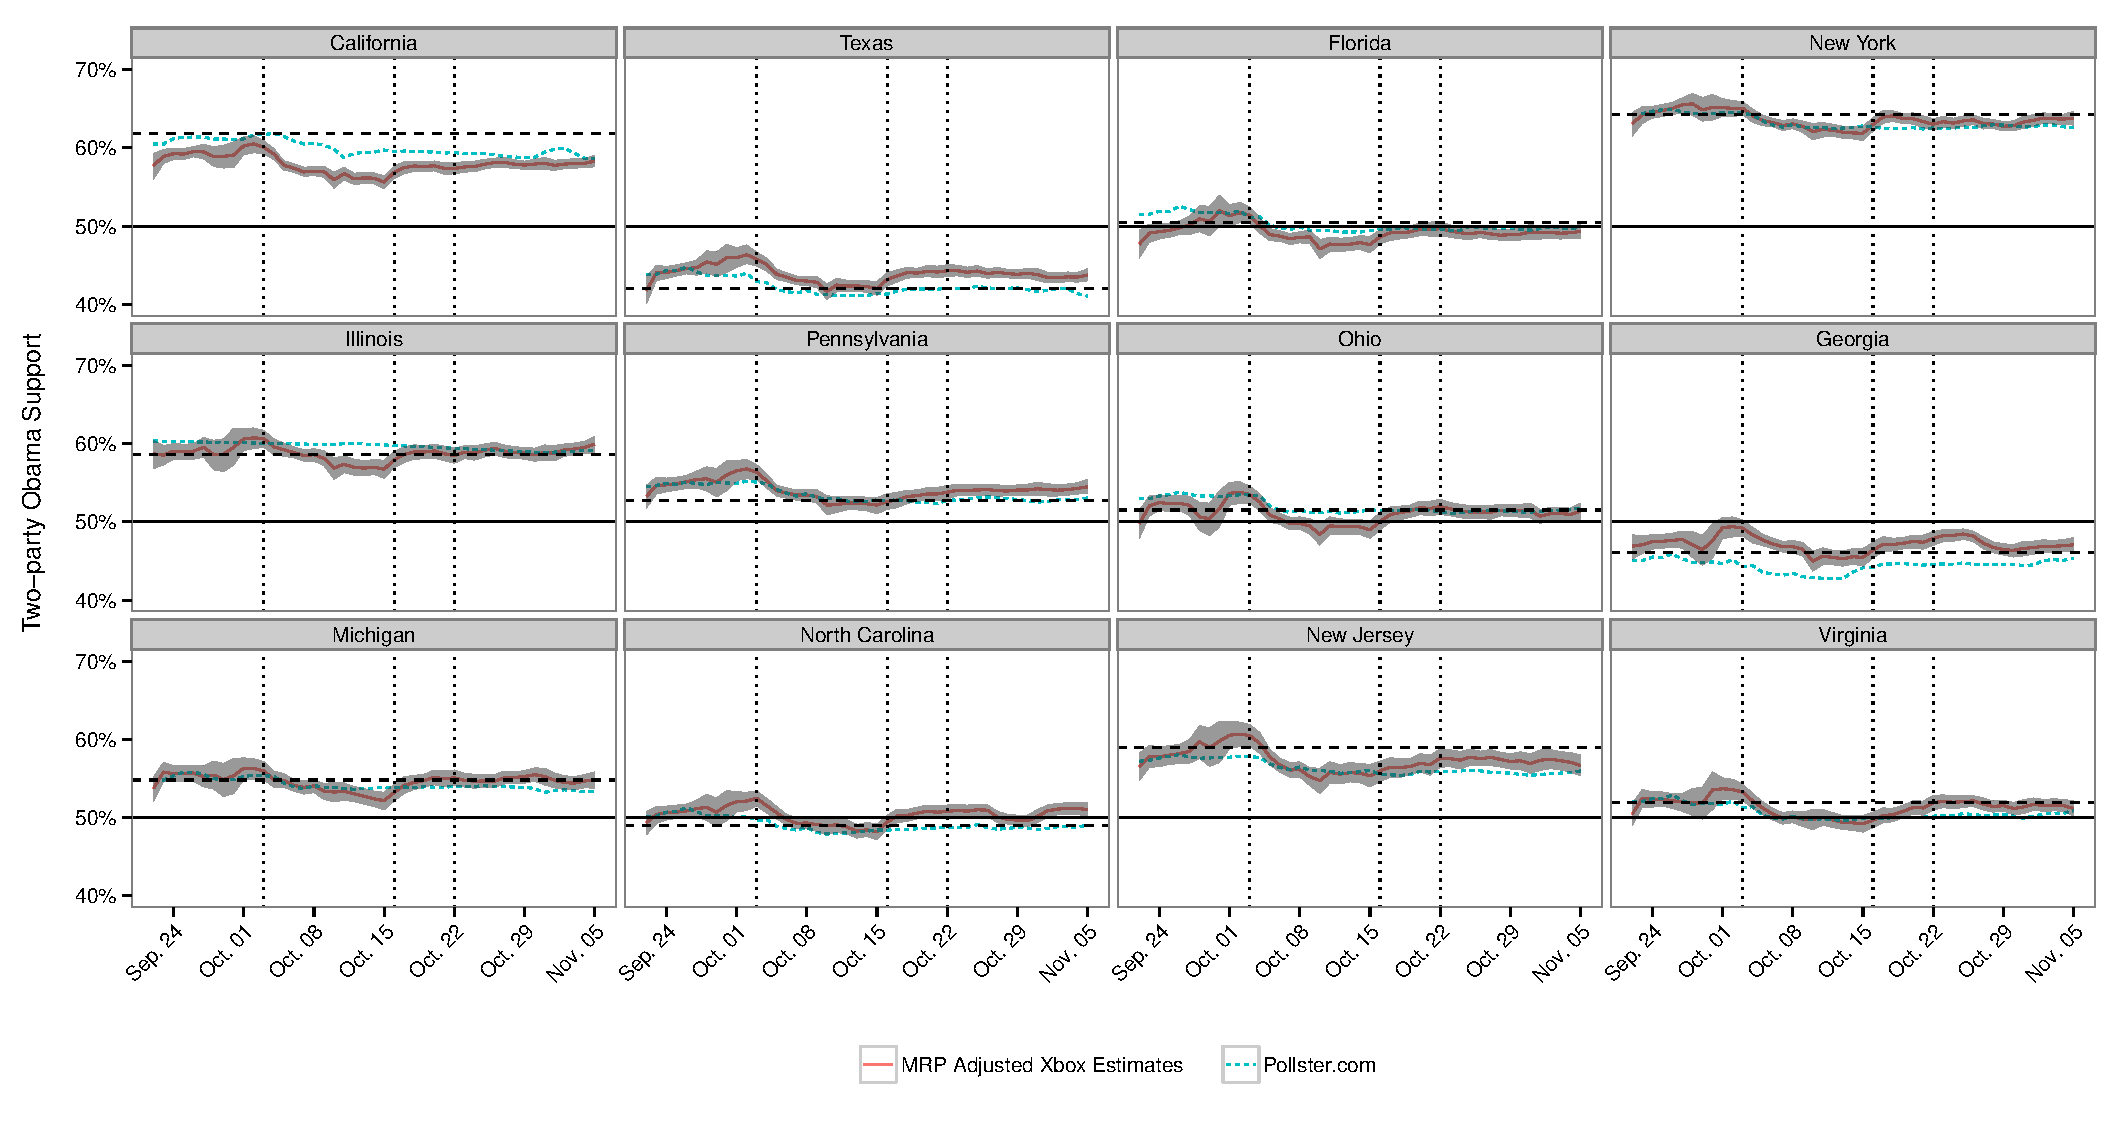
\includegraphics[width=15cm]{mrp_snapshots_state}
  \caption{MRP-adjusted daily voter intent for the 12 states with the most electoral
    votes, and the associated 95\% confidence bands. The horizontal dashed lines
    in each panel give the actual two-party Obama vote shares in that
    state. The mean and median absolute errors of the last day voter intent
    across the 51 Electoral College races are 2.5 and 1.8 percentage points,
    respectively. The state-by-state daily aggregated polling results from
    Pollster.com, given in the dotted blue lines, are broadly consistent with
    the estimates from the Xbox data.}
  \label{fig:state_snap}
\end{figure}

\subsection{Voter intent for demographic
subgroups}\label{voter-intent-for-demographic-subgroups}

Apart from Electoral College races, election forecasting often focuses
on candidate preference among demographic subpopulations. Such forecasts
are of significant importance in modern political campaigns, which often
employ targeted campaign strategies (Hillygus and Shields 2009). In the
highly non-representative Xbox survey, certain subpopulations are
heavily underrepresented and plausibly suffer from strong self-selection
problems. This begs the question, how accurate the estimates for older
women based on a platform that caters to mostly young men?

\begin{figure} \centering
  \includegraphics[width=\textwidth]{"demo_group_marginals"} \caption{Comparison
  of two-party Obama vote share for various demographic subgroups, as estimated
  from the 2012 national exit poll and from the Xbox data on the day before the
  election.  } \label{fig:marginal_comp} \end{figure}

\begin{figure}
  \centering
  \includegraphics[width=.6\textwidth]{"demo_groups_two_way_interaction"}
  \caption{Two-party Obama support as estimated from
  the 2012 national exit poll and from the Xbox data on the day before the election,
    for various two-way interaction demographic subgroups (e.g., 65+ year-old women).
    The sizes of the dots are proportional to the
    population sizes of the corresponding subgroups. Subgroups within the same
    two-way interaction category (e.g., age by sex) have the same color.}
  \label{fig:two_way_comp}
\end{figure}

It is straightforward in MRP to estimate voter intent among any
collection of demographic cells: I again use the same cell-level
estimates as in the national and state settings, but poststratify to the
desired target population. For example, to estimate voter intent among
women, the poststratification weights are based on the relative number
of women in each demographic cell. To illustrate this approach, I
compute Xbox estimates of Obama support for each level of the
categorical variables (e.g., males, females, Whites, Blacks, etc.) on
the day before the election, and compare those with the actual voting
behavior of those same groups as estimated by the 2012 national exit
poll. As seen in Figure\textasciitilde{}\ref{fig:marginal_comp}, the
Xbox estimates are remarkably accurate, with a median absolute
difference of 1.5 percentage points between the Xbox and the exit poll
numbers.\footnote{Respondents' 2008 vote was not asked on
the 2012 exit poll, so I exclude that comparison from
Figure~\ref{fig:marginal_comp}.}

Not only do the Xbox data facilitate accurate estimation of voter intent
across these single-dimensional demographic categories, but they also do
surprisingly well at estimating two-way interactions (e.g., candidate
support among 18--29 year-old Hispanics, and liberal college graduates).
Figure\textasciitilde{}\ref{fig:two_way_comp} shows this result,
plotting the Xbox estimates against those derived from the exit polling
data for each of the 149 two-dimensional demographic
subgroups.\footnote{State contestedness is excluded
from the two-way interaction groups since the 2012 state exit polls are not yet
available, and the 2012 national exit poll does not have enough data to reliably
estimate state interactions; 2008 vote is also excluded, as it was not asked in
the 2012 exit poll. The ``other'' race category was also dropped as it was not
consistently defined across the Xbox and exit poll datasets.} Most
points lie close to the diagonal, indicating that the Xbox and exit poll
estimates are in agreement. Specifically, for women who are 65 and
older---a group whose preferences one might a priori believe are hard to
estimate from the Xbox data---the difference between Xbox and the exit
poll is a mere one percentage point (49.5\% and 48.5\%, respectively).
Across all the two-way interaction groups, the median absolute
difference is just 2.4 percentage points. As indicated by the size of
the points in Figure\textasciitilde{}\ref{fig:two_way_comp}, the largest
differences occur for relatively small demographic subgroups (e.g.,
liberal Republicans), for which both the Xbox and exit poll estimates
are less reliable. For the 30 largest demographic subgroups,
Figure\textasciitilde{}\ref{fig:30groups} lists the differences between
Xbox and exit poll estimates. Among these largest subgroups, the median
absolute difference drops to just 1.9 percentage points.

\begin{figure}
  \centering
  \includegraphics{"two_way_interaction_diff"}
  \caption{Differences between the Xbox MRP-adjusted estimates and
    the exit poll estimates for the 30 largest two-dimensional demographic
    subgroups, ordered by the difference.  Positive values indicate the Xbox
    estimate is larger than the corresponding exit poll estimate.  Among these 30
    subgroups, the median and mean absolute differences are 1.9 and 2.2
    percentage points, respectively.}
  \label{fig:30groups}
\end{figure}

\section{Forecasting Election Day
Outcome}\label{forecasting-election-day-outcome}

\subsection{Converting Voter Intent to
Forecasts}\label{converting-voter-intent-to-forecasts}

As mentioned above, daily estimates of voter intent do not directly
correspond to estimates of vote share on election day. There are two key
factors for this deviation. First, opinion polls (both representative
and non-representative ones) only gauge voter preference on the
particular day when the poll is conducted, with the question typically
phrased as, ``if the election were held today.'' Political scientists
and pollsters have long observed that such stated preferences are prone
to several biases, including the anti-incumbency bias, in which the
incumbent's polling numbers tend to be lower than the ultimate outcome
(Campbell 2008), and the fading early lead bias, in which a big lead
early in the campaign tends to diminish as the election gets closer
(Erikson and Wlezien 2008). Moreover, voters' attitudes are affected by
information revealed over the course of the campaign, so preferences
weeks or months before election day are at best a noisy indicator of
one's eventual vote. Second, estimates of vote share require a model of
likely voters. That is, opinion polls measure preferences among a
hypothetical voter pool, and are thus accurate only to the extent that
this pool captures those who actually turn out to vote on election day.
Both of these factors introduce significant complications in forecasting
election day outcomes.

To convert daily estimates of voter intent to election day
predictions---which I hereafter refer to as ({\textbf{???}}) voter
intent---I compare daily voter intent in previous elections to the
ultimate outcomes in those elections. Specifically, I collected
historical data from three previous U.S. presidential elections, in
2000, 2004, and 2008. For each year, I obtained top-line (i.e., not
individual-level) national and state estimates of voter intent from all
available polls conducted in those elections.\footnote{I
collected the polling data from \url{Pollster.com} and
\url{RealClearPolitics.com}.} From this collection of polling data, I
then constructed daily estimates of voter intent by taking a moving
average of the poll numbers, in a similar manner to the major poll
aggregators. Note that I rely on traditional, representative polls to
reconstruct historical voter intent; in principle, however, I could have
started with non-representative polls if such data were available in
previous election cycles.

I next infer a mapping from voter intent to election outcomes by
regressing election day vote share on the historical time-series of
voter intent. The key difference between the approach in this chapter
and previous related work (Erikson and Wlezien 2008; Rothschild 2009) is
that I explicitly model state-level correlations, via nested national
and state models and correlated error terms. Specifically, I first fit a
national model given by

\begin{align*}
  y^{\text{US}}_{e}=a_0+a_1 x^{\text{US}}_{t,e}+
  a_2|x^{\text{US}}_{t,e}|x^{\text{US}}_{t,e} +
  a_3tx^{\text{US}}_{t,e} + \eta(t,e)
  \end{align*}

\noindent where \(y^{\text{US}}_{e}\) is the national election day vote
share of the incumbent party candidate in election year \(e\),
\(x^{\text{US}}_{t,e}\) is the national voter intent of the incumbent
party candidate at \(t\) days before the election in year \(e\), and
\(\eta \sim N(0,\sigma^2)\) is the error term. Both
\(y^{\text{US}}_{e}\) and \(x^{\text{US}}_{t,e}\) are offset by 0.5, so
the values run from \$-\$0.5 to 0.5 rather than 0 to 1. The term
involving the absolute value of voter intent pulls the vote share
prediction toward 50\%, capturing the diminishing early lead effect. I
do not include a main effect for time since it seems unlikely that the
number of days until the election itself contributes to the final vote
share directly, but rather time contributes through its interaction with
the voter intent (which it is include in the model).

Similarly, the state model is given by

\begin{align*}
  y_{s,e}^{\text{ST}}=b_0+b_1 x_{s,t,e}^{\text{ST}}+
  b_2|x_{s,t,e}^{\text{ST}}|x_{s,t,e}^{\text{ST}} +
  b_3tx_{s,t,e}^{\text{ST}} + \varepsilon(s,t,e)
\end{align*}

where \(y_{s,e}^{\text{ST}}\) is the election day state vote share of
the state's incumbent party
candidate\footnote{State incumbent parties are defined as the
  state-by-state winners from the previous election, which is more meaningful in this context than simply using the national incumbent.}
at day \(t\), \(x_{s,t,e}^{\text{ST}}\) is the state voter intent at day
\(t\), and \(\epsilon\) is the error term. The outcome
\(y_{s,e}^{\text{ST}}\) is offset by the national projected vote share
on that day as fit with the national calibration model, and
\(x_{s,t,e}^{\text{ST}}\) is offset by that day's national voter intent.
Furthermore, I impose two restrictions on the magnitude and correlation
structure of the error term \(\varepsilon(s,t,e)\). First, since the
uncertainty naturally decreases as the election gets closer (as \(t\)
becomes smaller), I apply the heteroscedastic structure
\(\text{Var}(\varepsilon(s,t,e))=(t+a)^2\), where \(a\) is a constant to
be estimated from the data. Second, the state-specific movements within
each election year are allowed to be correlated. For simplicity, and as
in (Chen, Ingersoll, and Kaplan 2008), I assume these correlations are
uniform (i.e., all pairwise correlations are the same), which creates
one more parameter to be estimated from the data. I fit the full
calibration model with the \texttt{gls()} function in the \texttt{R}
package \texttt{nlme} (Pinheiro et al. 2012).

In summary, the procedure for generating election day forecasts proceeds
in three steps:

\begin{enumerate}
\item Estimate the joint distribution of state and national voter intent by applying MRP to the Xbox data,
as described in Section~\ref{sec:mrp}.
\item Fit the nested calibration model described above on historical data to obtain point estimates for the parameters, including
estimates for the error terms.
\item Convert the distribution of voter intent to election day forecasts via the fitted calibration model.
\end{enumerate}

\subsection{National and state election day
forecasts}\label{national-and-state-election-day-forecasts}

Figure \ref{fig:proj_state} plots the projected vote shares and
pointwise 95\% confidence bands over time for the 12 states with the
most electoral votes. Though these time-series look quite reasonable, it
is difficult to assess their accuracy as there are no ground truth
estimates to compare with in the weeks prior to the election. As a
starting point, I compare the state-level estimates to those generated
by prediction markets, which are widely considered to be among the most
accurate sources for political predictions\textasciitilde{}(Rothschild
2013; Wolfers and Zitzewitz 2004). For each state, prediction markets
produce daily probabilities of victory. Though
Figure\textasciitilde{}\ref{fig:proj_state} plots the forecasts in terms
of expected vote share, this estimation procedure in fact yields the
full distribution of outcomes, and so I can likewise convert my
estimates to probabilistic forecasts.
Figure\textasciitilde{}\ref{fig:pm_comp} shows this comparison, where
the prediction market estimate is derived by averaging the two largest
election markets, Betfair and Intrade. My probabilistic estimates are
largely consistent with the prediction market probabilities. In fact,
for races with little uncertainty (e.g., Texas and Massachusetts), the
Xbox estimates do not seem to suffer from the long-shot bias common to
prediction markets (Rothschild 2009), and instead yield probabilities
closer to 0 or 1. For tighter races, the Xbox estimates---although still
highly correlated with the prediction market probabilities---look more
volatile, especially in the early part of the 45-day period. Since the
ground truth is not clearly defined, it is difficult to evaluate which
method---Xbox or prediction markets---yields better results. From a
Bayesian perspective, if one believes the stability shown by prediction
markets, this could be incorporated into the structure of the Xbox
calibration model.

\begin{figure}[p!]
  \centering
  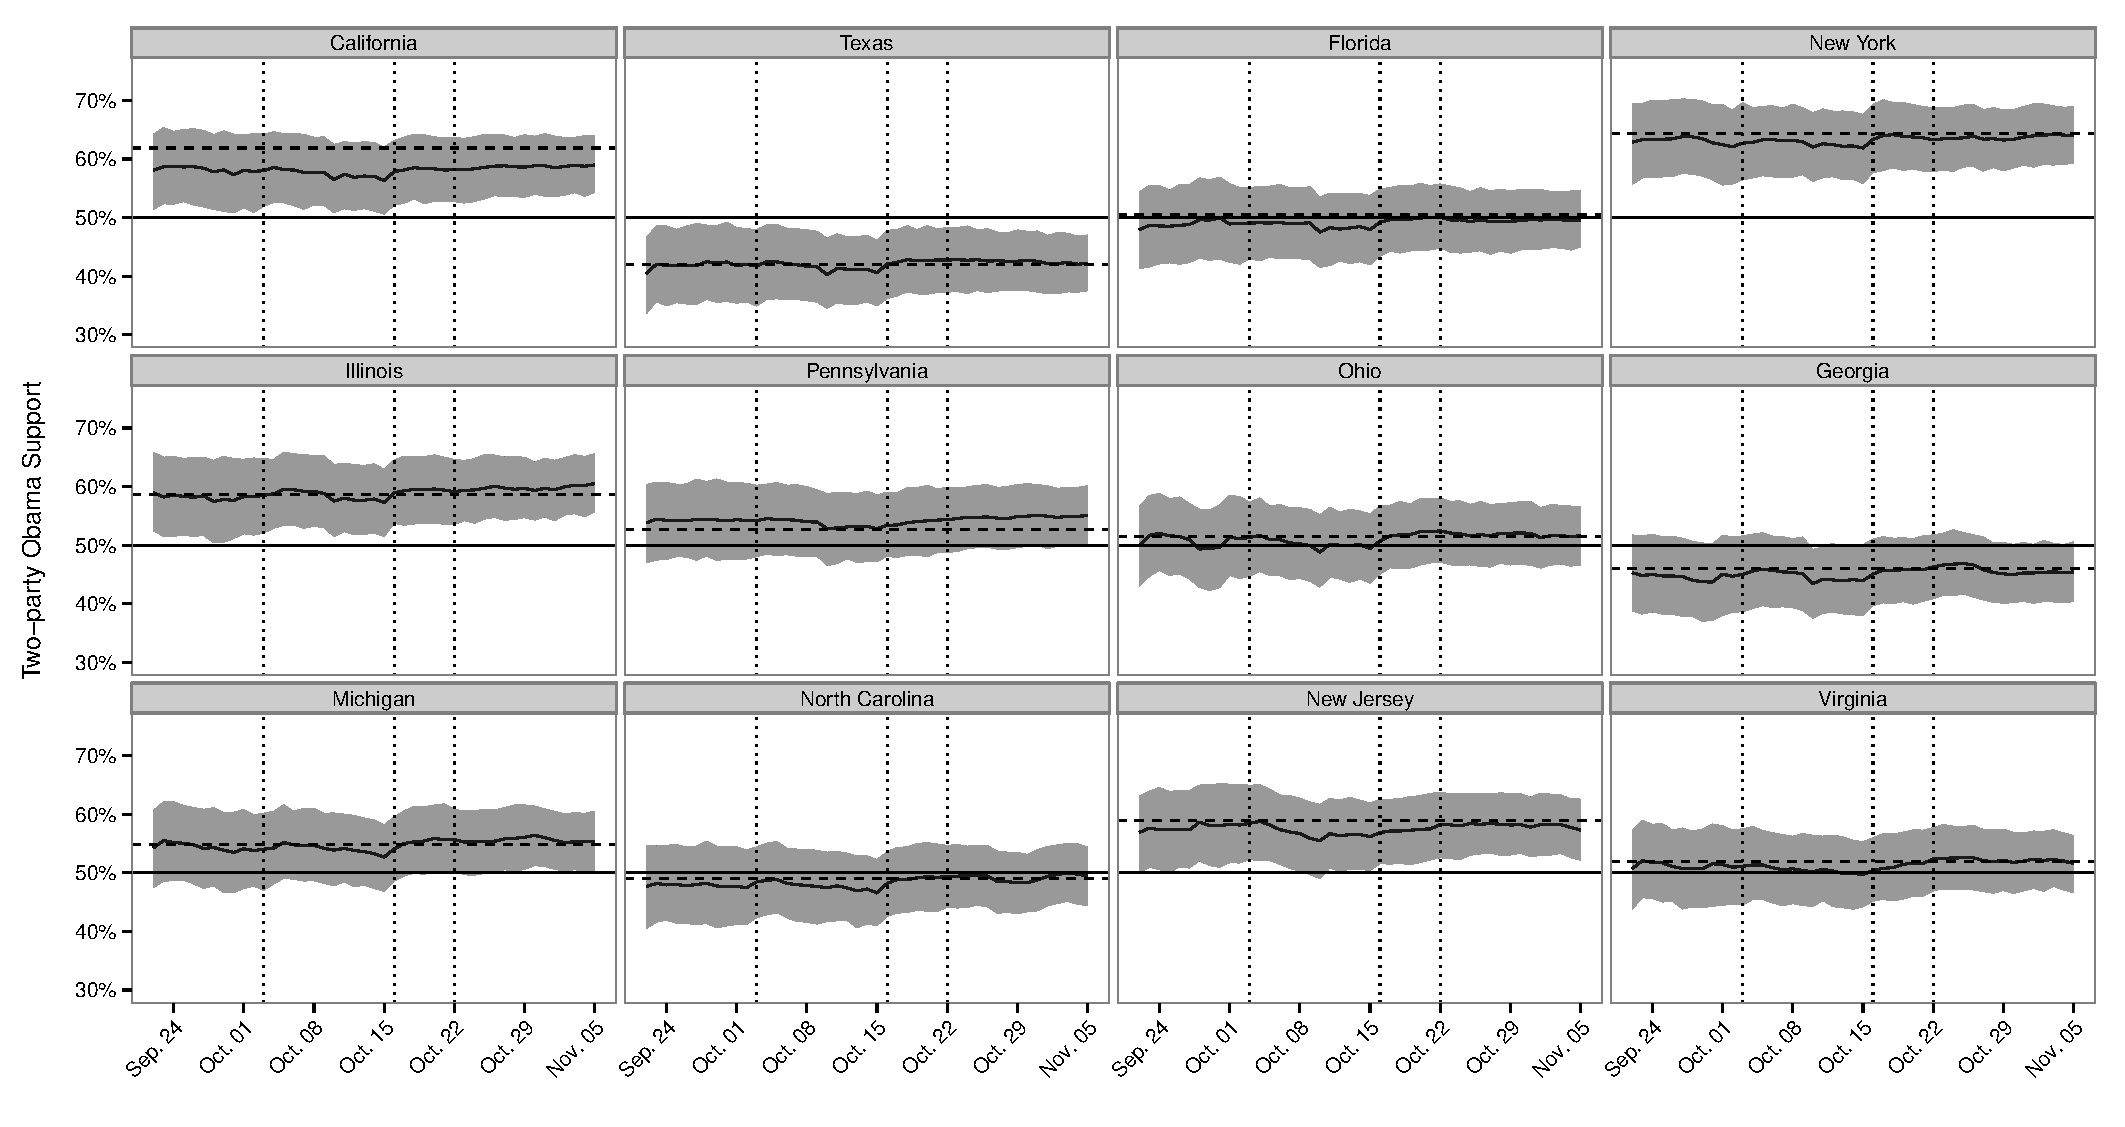
\includegraphics[width=\textwidth]{projected_voteshare_state}
  \caption{Projected Obama share of the two-party vote on election day
    for each of the 12 states
    with the most electoral votes, and associated 95\% confidence
    bands. Compared to the MRP-adjusted voter intent in Figure
    \ref{fig:state_snap}, the projected two-party Obama support is more stable, and the North Carolina race switches direction after applying the
    calibration model. Additionally, the confidence bands become much wider and
    give more reasonable state-by-state probabilities of Obama victories.}
  \label{fig:proj_state}
\end{figure}

\begin{figure}[p!]
  \centering
  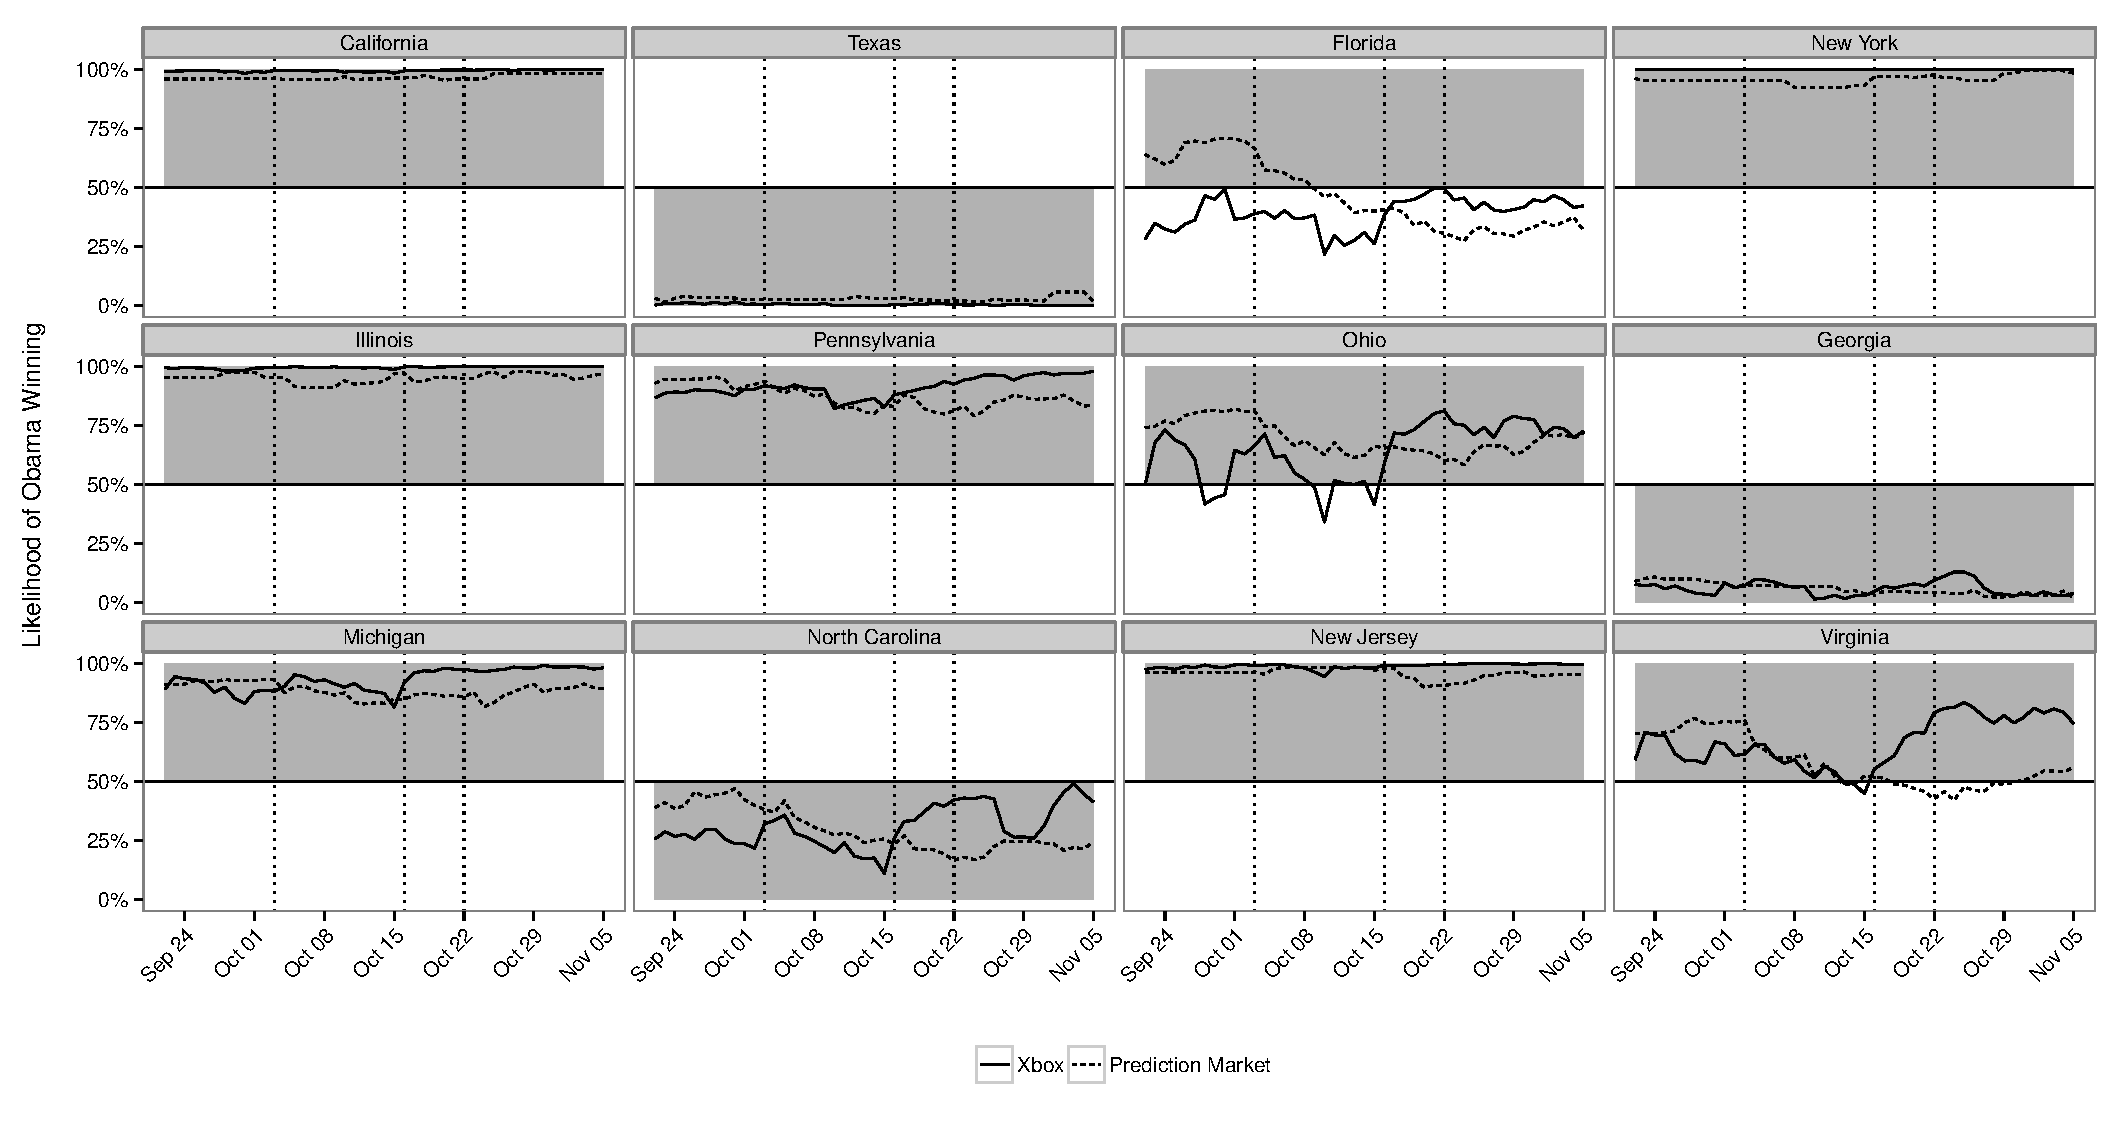
\includegraphics[width=\textwidth]{pred_market_xbox_comp}
  \caption{Comparison between the probability of Obama winning the 12 largest
    Electoral College races based on Xbox data and on prediction market
    data. The prediction market data are the average of the raw Betfair and Intrade
    prices from winner-take-all markets. The three vertical lines represent the
    dates of three presidential debates. The shaded halves indicate the direction
    that race went.}
  \label{fig:pm_comp}
\end{figure}

\begin{figure}[p!]
  \centering
  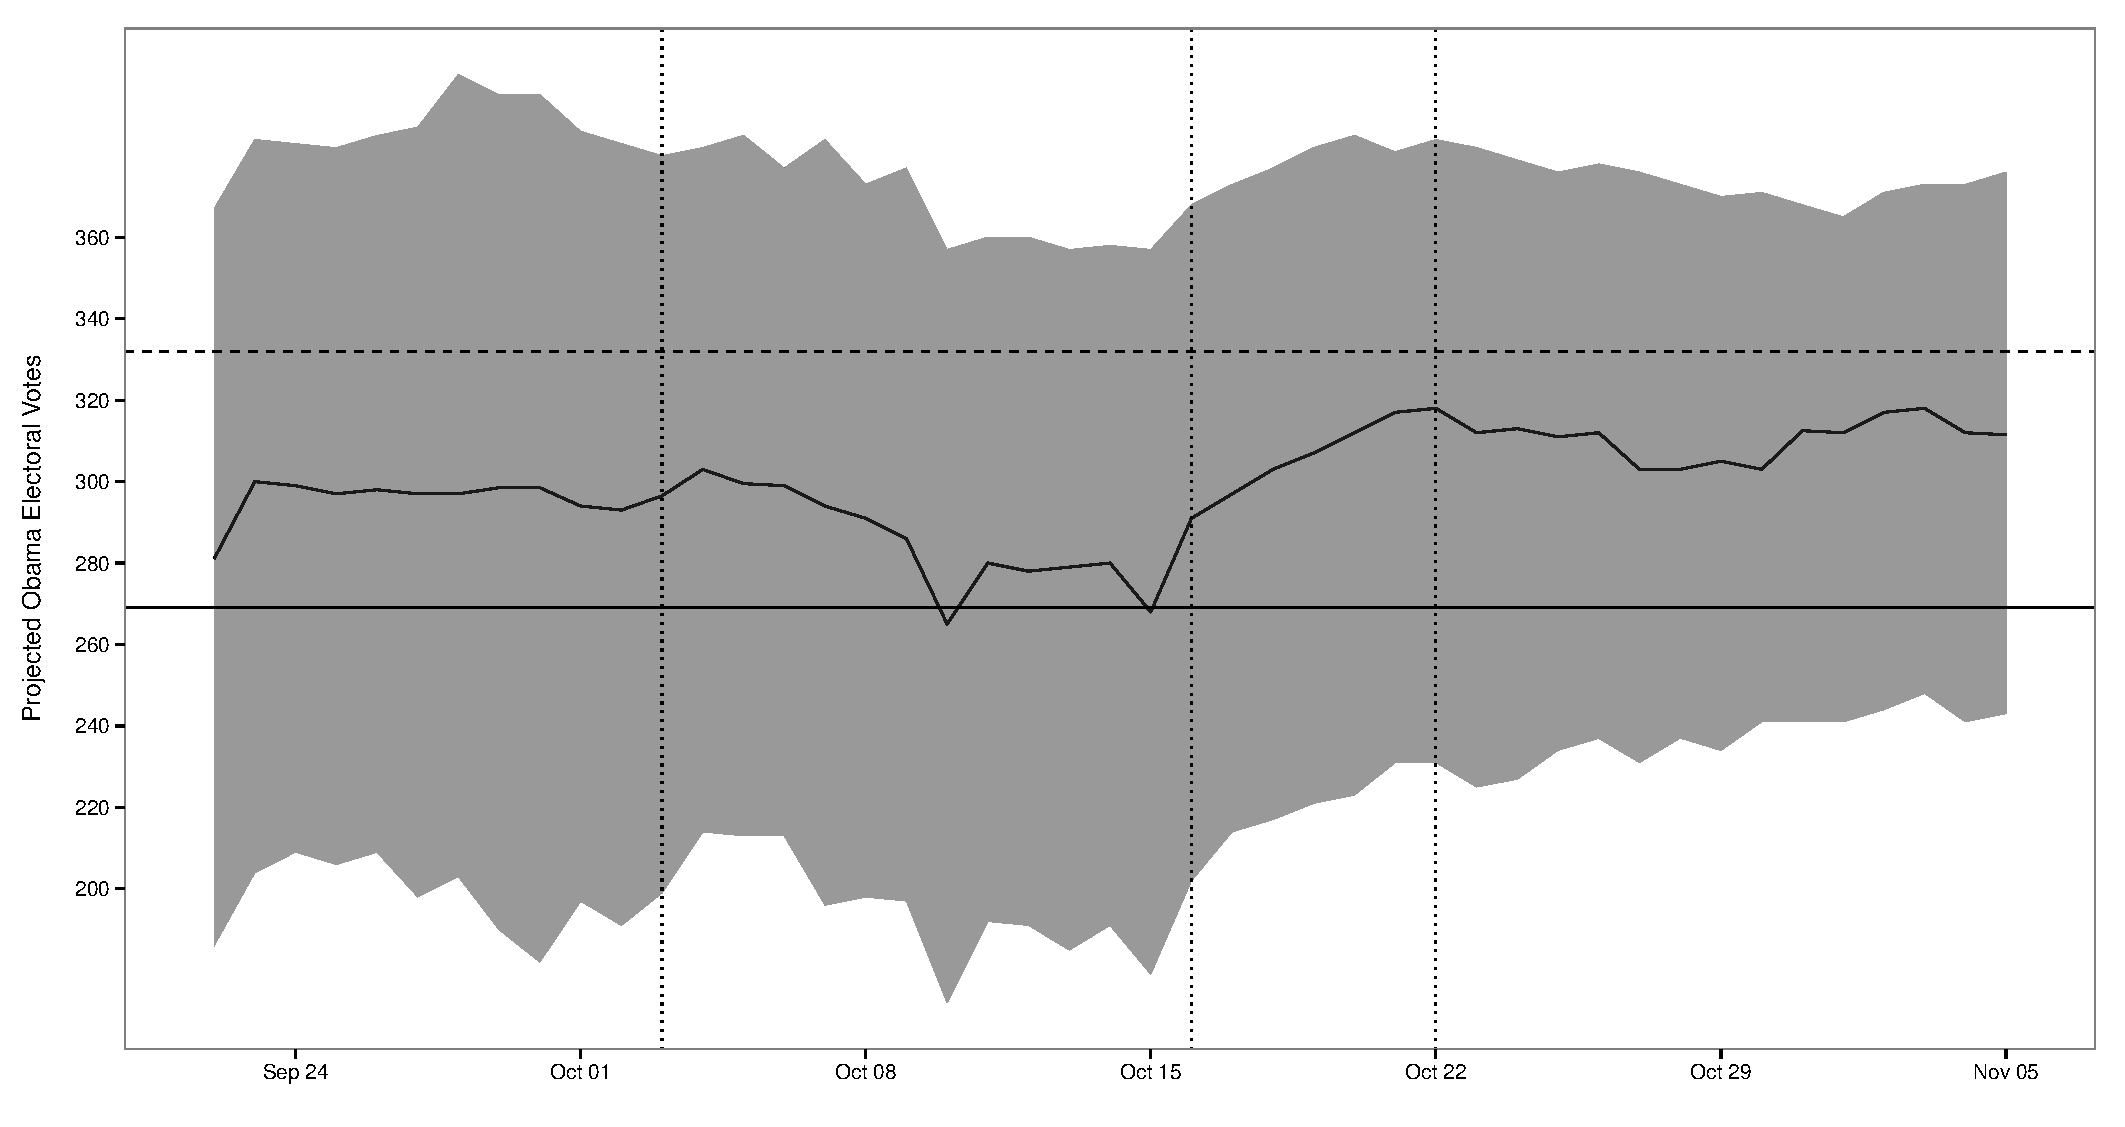
\includegraphics[width=\textwidth]{electoral_vote_dist_over_time}
  \caption{Daily projections of Obama electoral votes in the 45-day period
    leading up to the 2012 election and associated 95\% confidence bands. The
    solid line represents the median of the daily distribution. The horizontal
    dashed line represents the actual electoral votes, 332, that Obama captured
    in 2012 election. Three vertical dotted lines indicate the dates of three
    presidential debates.}
  \label{fig:ev_daily}
\end{figure}

\begin{figure}[p!]
  \centering
  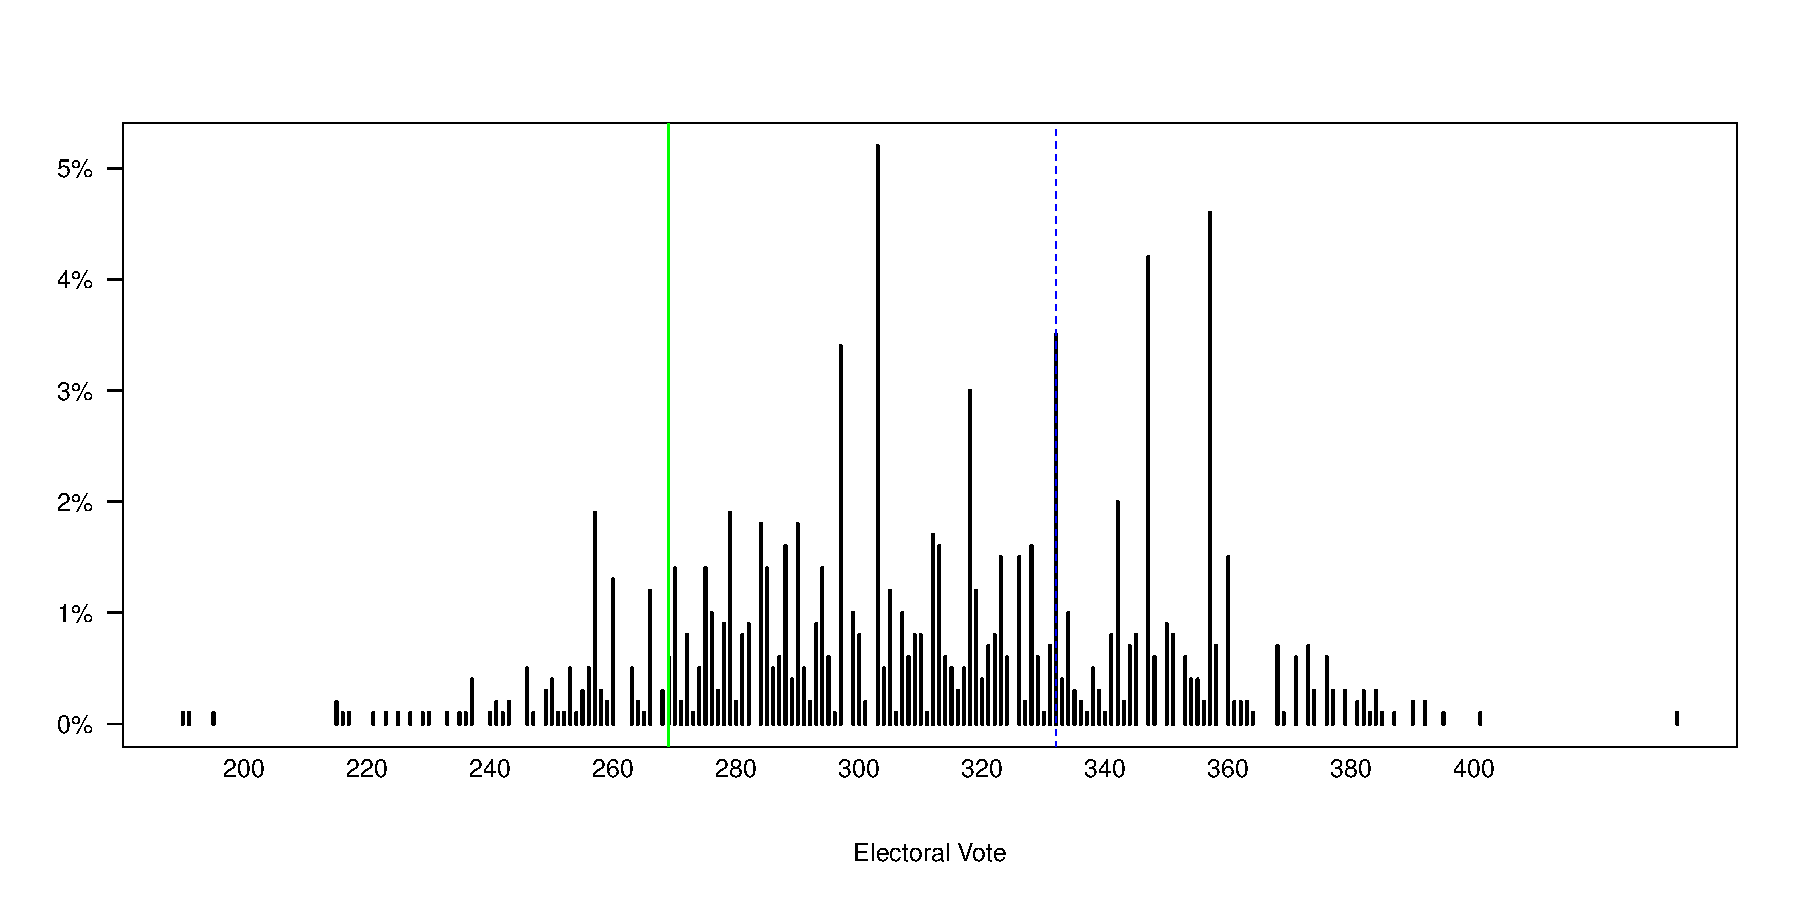
\includegraphics[width=\textwidth]{last_day_electoral_vote_dist}
  \caption{Projected distribution of electoral votes for Obama one day before the election. The green vertical dotted line represents 269, the minimum number of electoral votes that Obama needs for a tie. The blue vertical dashed line gives 332, the actual number of electoral votes captured by Obama. The estimated likelihood of Obama winning the electoral vote is 88\%.}
  \label{fig:ev_lastday}
\end{figure}

With the full state-level outcome distribution, I can also estimate the
distribution of Electoral College votes.
Figure\textasciitilde{}\ref{fig:ev_daily} plots the median projected
electoral votes for Obama over the last 45-days of the election,
together with the 95\% confidence band. In particular, on the day before
the election, my model estimates Obama had an 88\% chance of victory, in
line with estimates based on traditional polling data. For example,
Simon Jackman predicted Obama had a 91\% chance of victory, using a
method built from (Jackman 2005). Zooming in on the day before the
election, Figure\textasciitilde{}\ref{fig:ev_lastday} shows the full
predicted distribution of electoral votes for Obama. Compared to the
actual 332 votes that Obama captured, I estimate a median of 312 votes,
with the most likely outcome being 303. Though this distribution of
Electoral College outcomes seems reasonable, it does appear to have
higher variance than one might expect. In particular, the extreme
outcomes seem to have unrealistically high likelihood of occurring,
which is likely a byproduct of the calibration model not fully capturing
the state-level correlation structure. Nonetheless, given that my
forecasts are based on a highly biased convenience sample of
respondents, the model predictions are remarkably good.

\section{Conclusion}\label{conclusion}

Forecasts not only need to be accurate, but also relevant, timely, and
cost-effective. In this chapter, I construct election forecasts
satisfying all of these requirements using extremely non-representative
data. Though the data were collected on a proprietary polling platform,
in principle one can aggregate such non-representative samples at a
fraction of the cost of conventional survey designs. Moreover, the data
produce forecasts that are both relevant and timely, as they can be
updated faster and more regularly than standard election polls. Thus,
the key question---and one of the main contributions of this
chapter---is to assess the extent to which one can generate accurate
predictions from non-representative samples. Since there is limited
ground truth for election forecasts, definitely establishing the
accuracy of my predictions is difficult. Nevertheless, I show that the
MRP-adjusted and calibrated Xbox estimates are both intuitively
reasonably, and are also quite similar to those generated by more
traditional means.

The greatest impact of non-representative polling will likely not be for
presidential elections, but rather for smaller, local elections and
specialized survey settings, where it is impractical to deploy
traditional methods due to cost and time constraints. For example,
non-representative polls could be used in Congressional elections, where
there are currently only sparse polling data. Non-representative polls
could also supplement traditional surveys (e.g., the General Social
Survey) by offering preliminary results at shorter intervals. General
Social Survey, which is . Finally, when there is a need to identify and
track pivotal events that affect public opinion, non-representative
polling offers the possibility of cost-effective continuous data
collection. Standard representative polling will certainly continue to
be an invaluable tool for the foreseeable future. However, 75 years
after the \textsl{Literary Digest} failure, non-representative polling
(followed by appropriate post-data adjustment) is due for further
exploration, for election forecasting and in social research more
generally.

\hyperdef{}{references}{\label{references}}
\section*{Bibliography}\label{bibliography}
\addcontentsline{toc}{section}{Bibliography}

\hyperdef{}{ref-bates2013lme4}{\label{ref-bates2013lme4}}
Bates, Douglas, Martin Maechler, and Ben Bolker. 2013. \emph{Lme4:
Linear mixed-effects models using s4 classes}.
\url{http://CRAN.R-project.org/package=lme4}.

\hyperdef{}{ref-campbell2008american}{\label{ref-campbell2008american}}
Campbell, James E. 2008. 6 \emph{The american campaign: US presidential
campaigns and the national vote}. Texas A\&M University Press.

\hyperdef{}{ref-chen2008modeling}{\label{ref-chen2008modeling}}
Chen, M Keith, Jonathan E Ingersoll, and Edward H Kaplan. 2008.
``Modeling a presidential prediction market.'' \emph{Management Science}
54(8): 1381--1394.

\hyperdef{}{ref-erikson2008political}{\label{ref-erikson2008political}}
Erikson, Robert S, and Christopher Wlezien. 2008. ``Are political
markets really superior to polls as election predictors?'' \emph{Public
Opinion Quarterly} 72(2): 190--215.

\hyperdef{}{ref-gelman2007data}{\label{ref-gelman2007data}}
Gelman, Andrew, and Jennifer Hill. 2007. \emph{Data analysis using
regression and multilevel/hierarchical models}. Cambridge University
Press.

\hyperdef{}{ref-ghitzaux5f2013}{\label{ref-ghitzaux5f2013}}
Ghitza, Yair, and Andrew Gelman. 2013. ``Deep interactions with mRP:
Election turnout and voting patterns among small electoral subgroups.''
\emph{American Journal of Political Science} 57(3): 762--776.

\hyperdef{}{ref-gosnell1937technical}{\label{ref-gosnell1937technical}}
Gosnell, Harold F. 1937. ``How accurate were the polls?'' \emph{Public
Opinion Quarterly} 1(1): 97--105.

\hyperdef{}{ref-hillygus2009persuadable}{\label{ref-hillygus2009persuadable}}
Hillygus, D Sunshine, and Todd G Shields. 2009. \emph{The persuadable
voter: Wedge issues in presidential campaigns}. Princeton University
Press.

\hyperdef{}{ref-jackman2005pooling}{\label{ref-jackman2005pooling}}
Jackman, Simon. 2005. ``Pooling the polls over an election campaign.''
\emph{Australian Journal of Political Science} 40(4): 499--517.

\hyperdef{}{ref-kaufmann1999changing}{\label{ref-kaufmann1999changing}}
Kaufmann, Karen M, and John R Petrocik. 1999. ``The changing politics of
american men: Understanding the sources of the gender gap.''
\emph{American Journal of Political Science} 43(3): 864--887.

\hyperdef{}{ref-keeter2006gauging}{\label{ref-keeter2006gauging}}
Keeter, Scott et al. 2006. ``Gauging the impact of growing nonresponse
on estimates from a national rDD telephone survey.'' \emph{Public
Opinion Quarterly} 70(5): 759--779.

\hyperdef{}{ref-kohut2012assessing}{\label{ref-kohut2012assessing}}
Kohut, Andrew et al. 2012. ``Assessing the representativeness of public
opinion surveys.'' \emph{Pew Research Center for The People \& The
Press} 15(May): 2012.

\hyperdef{}{ref-laxux5f2009}{\label{ref-laxux5f2009}}
Lax, Jeffrey R, and Justin H Phillips. 2009. ``How should we estimate
public opinion in the states?'' \emph{American Journal of Political
Science} 53(1): 107--121.

\hyperdef{}{ref-little1993post}{\label{ref-little1993post}}
Little, Roderick JA. 1993. ``Post-stratification: A modeler's
perspective.'' \emph{Journal of the American Statistical Association}
88(423): 1001--1012.

\hyperdef{}{ref-lockux5f2010}{\label{ref-lockux5f2010}}
Lock, Kari, and Andrew Gelman. 2010. ``Bayesian combination of state
polls and election forecasts.'' \emph{Political Analysis} 18(3):
337--348.

\hyperdef{}{ref-park2004bayesian}{\label{ref-park2004bayesian}}
Park, David K, Andrew Gelman, and Joseph Bafumi. 2004. ``Bayesian
multilevel estimation with poststratification: State-level estimates
from national polls.'' \emph{Political Analysis} 12(4): 375--385.

\hyperdef{}{ref-nlme}{\label{ref-nlme}}
Pinheiro, Jose et al. 2012. \emph{Nlme: Linear and nonlinear mixed
effects models}.

\hyperdef{}{ref-rothschild2013combining}{\label{ref-rothschild2013combining}}
Rothschild, David. 2013. ``Combining forecasts: Accurate, relevant, and
timely.''

\hyperdef{}{ref-rothschild2009forecasting}{\label{ref-rothschild2009forecasting}}
Rothschild, David. 2009. ``Forecasting elections comparing prediction
markets, polls, and their biases.'' \emph{Public Opinion Quarterly}
73(5): 895--916.

\hyperdef{}{ref-squire19881936}{\label{ref-squire19881936}}
Squire, Peverill. 1988. ``Why the 1936 literary digest poll failed.''
\emph{Public Opinion Quarterly} 52(1): 125--133.

\hyperdef{}{ref-wang2014forecasting}{\label{ref-wang2014forecasting}}
Wang, Wei et al. 2014. ``Forecasting elections with non-representative
polls.'' \emph{International Journal of Forecasting}.

\hyperdef{}{ref-wolfers2004prediction}{\label{ref-wolfers2004prediction}}
Wolfers, Justin, and Eric Zitzewitz. 2004. \emph{Prediction markets}.
National Bureau of Economic Research.


\part{Causal Inference of Meta-anlaysis}
\label{sec:meta}
\chapter{Causal Inference of Meta-Analysis via Gaussian Processess}

Meta-Analysis, the synthesis of evidence from multiple study sources,
has become increasing popular in fields such as education, psychology
and public health (Cooper, Hedges, and Valentine 2009). The major
obstacle for meta-analysis is the interpretation and proper handling of
study-by-study heterogeneity, e.g., the estimated treatment effect in
study 1 is different from in study 2. Traditional approaches tend to
focus on developing novel ways of weighting different estimates based on
certain measure of study-level uncertainty and/or quality. (Sobel,
Madigan, and Wang 2016), however, approaches this problem from a formal
causal inference perspective, proposing an extended potential outcome
framework for meta-analysis. Although it is not a panacea for explaining
and accounting for heterogeneities, this approach indeed clarifies the
originations of heterogeneities and help researchers to think more
clearly on underlying assumptions that are often overlooked. In this
chapter, I review briefly the extended potential outcome framework
discussed in (Sobel, Madigan, and Wang 2016). However, (Sobel, Madigan,
and Wang 2016) use simple linear models for analysis. In remaining part
of this thesis, I develop a non-parametric model that explicitly handles
heterogeneities across studies based on Gaussian Processes (GP). As it
is well known (Williams and Rasmussen 2006), GP allows for flexible
modeling of response functions and admits fully probabilistic inference.
Finally, a real educational intervention data set is analyzed with this
model to illustrate. This chapter is joint work with Michael Sobel and
David Madigan, and part of it is published in (Sobel, Madigan, and Wang
2016).

\section{Meta-Analysis}\label{meta-analysis}

Meta-analyses combine data from distinct but related studies for higher
resolution inference and more nuanced understanding of the effect under
investigation. Originally hailed in medical and education research,
meta-analyses are gaining traction as the awareness for open data is
increasing across all scientific communities.

However, traditional meta-analyses are mostly conducted based on
extracting and combining study-level effect summaries, since access to
individual-participant level data tend to be inherently difficult to
obtain. In this framework, researchers extract effect size estimates
\(y_s\) and standard errors \(\sigma_s^2\), where study index
\(s\in \{1,\ldots,S\}\) and \(S\) is the total number of studies. To
handle effect size heterogeneity, typically a random effect model is
used (DerSimonian and Laird 1986), in which all study effect sizes are
assumed to be a random sample of a underlying hyper-population of effect
sizes, i.e.

\begin{align*}
    y_s&=\mu_s + \sigma_s^2\\
    \mu_s &\sim \mathcal{N}(\mu_0, \tau^2)
\end{align*}

\noindent Admittedly, meta-analysis based on study-level summary is
still effective when the effects are homogeneous and different studies
sample from similar populations; nevertheless, they are prone to
well-known statistical fallacies, such as ecological bias, when the
underlying populations and effects are heterogeneous, as it is often the
case in real data.

\subsection{Individual-Participant
Meta-Analyses}\label{individual-participant-meta-analyses}

Individual-Participant Data (IPD) Meta-Analyses are becoming more and
more common, thanks to the increasing availability of original data
(Higgins et al. 2001). It has been argued that IPD data increases the
power of analysis (Cooper and Patall 2009) and more robust to
heterogeneous effects sizes and populations. To account for between
study heterogeneity in treatment effects, the use of covariates and/or
random effects models is often recommended (Aitkin 1999; Tudur Smith,
Williamson, and Marson 2005). The random effects models can be seen as
Bayesian hierarchical models (Gelman and Hill 2006), based on the
justification that conditioned on an appropriate set of covariates, both
individual-level and study-level, the residual heterogeneities are
exchangeable. There are mature softwares for fitting various types of
Bayesian hierarchical models, including Generalized Linear Models and
Proportional Hazard Models (Bates et al. 2015; ``Stan: A c++ library for
probability and sampling, version 2.8.0'' 2015; Therneau 2012).

Despite its convenient form and ease of inference, traditional IPD
meta-analysis based on parametric hierarchical models suffer from two
problems. The first is the lack of formal causal framework. It is
difficult to pinpoint the causal interpretation of the effect estimates
from a traditional IPD hierarchical model. Consider the following
example, education researchers try to determine the effect of a new
intervention program, applied to different classroom and administered by
different teachers. In this case, the heterogeneity might come from
either the different teachers or the different populations of schools,
or both. It is often unclear whether the effect estimate based on
traditional methods are averages over the teachers, or over the schools,
or both. The second problem is the inflexible form of the parametric
model. Traditional parametric model requires explicit modeling
assumptions from the researchers, which makes the model sensitive to
model specifications and facilitate potential cheery-picking.
Non-parametric modeling allows flexible functional form and requires
little manual tuning from the researchers.

\section{A Potential Outcome Framework for
Meta-Analysis}\label{a-potential-outcome-framework-for-meta-analysis}

(Sobel, Madigan, and Wang 2016) put meta-analysis on a concrete causal
foundation by introducing an extended potential outcome framework. I
will discuss the key ideas in this framework.

\subsection{Potential Outcomes}\label{potential-outcomes}

Potential Outcomes Framework (Rubin 2011) defines causal effects as
comparisons of outcomes under hypothetical counter-factual treatment
assignment. For example, with binary treatment \(Z\in \{0,1\}\), the
causal effect of treatment \(Z\) on individual \(i\) can be defined as
\(y_i(1)-y_i(0)\). Typically, researchers are interested in estimating
quantities such as the population average treatment effect (PATE)

\begin{equation*} E(Y(1)-Y(0)), \end{equation*}

\noindent and the population average treatment effect on the treated
(PATT)

\begin{equation*}
    E(Y(1)-Y(0)\mid Z=1)
\end{equation*}

\noindent The key assumption in causal inference is the ignorability
assumption (or unconfoundedness assumption) (Rosenbaum and Rubin 1983),
which states that given a set of observed covariates, the treatment
assignment \(Z\) is independent of the potential outcomes
\((Y(0), Y(1))\)

\begin{equation*}
    Y(0),Y(1) \perp Z \mid X
\end{equation*}

\noindent In the case of randomized experiment, this assumption is
trivially met without any covariates \(X\). Under ignorability
assumption,

\begin{align*}
     &E(Y|X, z=1)-E(Y|X, z=0)\\
    =&E(Y(1)|X, z=1)-E(Y(0)|X, z=0)\\
    =&E(Y(1)|X)-E(Y(0)|X)\\
    =&E(Y(1)-Y(0)|X)
\end{align*}

\noindent and thus causal effect can be identified from observations.

\subsection{Extended Potential
Outcomes}\label{extended-potential-outcomes}

In the case of meta-analysis, consisting \(S\) studies and \(Z\)
treatment arms, the potential outcomes \(\bm Y\) for individual \(i\)
can be defined as a matrix

\begin{equation*}
\bm Y_i=
\begin{pmatrix}
y_i(1,1) & y_i(1,2) & \cdots & y_i(1,Z)\\
y_i(2,1) & y_i(2,2) & \cdots & y_i(2,Z)\\
\vdots & \vdots & \ddots & \vdots\\
y_i(S,1) & y_i(S,2) & \cdots & y_i(S,Z)
\end{pmatrix}
\end{equation*}

\noindent With this notation, some commonly discussed meta-analytical
estimates can be interpreted in a causal way. For example, assuming
there are only two level of treatment (0 and 1) and the causal
comparison is the difference, \emph{study-specific} treatment effect for
study \(s\) is \(E(y(z,s)-y(z^\prime, s))\). Note that this is different
from \emph{study-level} treatment effect \(\theta_s\) in random effects
models, which is \(E(y(z,s)-y(z^\prime, s)\mid S=s)\). Below I will
discuss conditions that will connect these two quantities.

In the context of meta-analyses, unconfoundedness can be recast as
unconfoundedness within each study, i.e.,

\begin{equation*}
    Y(0, s),Y(1, s) \perp Z \mid X, S=s
\end{equation*}

However, this assumption is not sufficient for identifying causal
effects in meta-analysis. One added layer for complexity of
meta-analysis is the confounding of study selection. Consider an example
of clinical trials. If some studies sample from mostly young patients
while some other studies sample from mostly elderly patients, and the
treatment is more effective on younger patients, then heterogeneities in
treatment effects across studies would arise. Hierarchal models without
adequately addressing this selection problems would result in misleading
results.

However, study selection is not the only factor contributing to
heterogeneities in treatment effects across studies. One lingering
question is whether the same treatment \(z\) is implemented identically
in all studies, or in another word, whether
\(Y_i(s_1, z)\disteq Y_i(s_2, z)\) for all pair of
\(s_1, s_2 \in \{1,\dots, S\}\), where \(\disteq\) stands for equal in
distribution. Consider an example of education intervention, in which
interventions are carried out by teachers with various experience
levels, then it is reasonable to question whether
\(Y_i(s_1, z)\disteq Y_i(s_2, z)\) holds.

Two assumptions from (Sobel, Madigan, and Wang 2016) codify these two
sources of heterogeneities.

A1. \emph{Weak response consistency assumption for treatment \(z\)}: For
any \(z\in\{1,\dots,Z\}\) and any pair \(s_1, s_2\in\{1,\ldots,S\}\),

\begin{equation*}
Y_i(s_1, z)\disteq Y_i(s_2, z)
\end{equation*}

A2. \emph{Unconfounded study selection}:

\begin{equation*}\bm Y=
\begin{pmatrix}
y(1,1) & y(1,2) & \cdots & y(1,Z)\\
y(2,1) & y(2,2) & \cdots & y(2,Z)\\
\vdots & \vdots & \ddots & \vdots\\
y(S,1) & y(S,2) & \cdots & y(S,Z)
\end{pmatrix}
 \perp S \mid X\end{equation*}

.

From a modeling perspective, these two assumptions cannot be
distinguished from one other. Thus (Sobel, Madigan, and Wang 2016)
suggests that researchers first assess the plausibility of the two
assumptions based on the characteristics of the studies, and typically
assume one of these two to hold and then build models to see whether the
heterogeneity could be accounted for by the other assumption. From a
Bayesian point of view, I can use a very general model, and encode
regularization through appropriate prior distributions to allow for
reasonable separation of these two sources of heterogeneities. This will
be the topic of the following sections.

\section{Meta-Analysis using Bayesian
Non-parametrics}\label{meta-analysis-using-bayesian-non-parametrics}

Traditionally, causal inference using potential outcomes focuses on two
questions. Modeling of the treatment assignment process \(p(z\mid x)\),
also known as the propensity score, and modeling of the scientific
process of how responses relate to treatment and covariates
\(p(y\mid z, x)\), also known as the response surface (Rubin 2005). A
myriad of methods based on the either treatment assignment mechanism
(e.g., propensity score matching), or response surface modeling (e.g.,
regression), or combination of these two (e.g., the doubly-robust
method), has been proposed for causal inference of observational data.

Recently, following the advances in Bayesian non-parametric models ,
(Hill 2011) proposed a model that focuses on accurately estimating the
response surface using flexible Bayesian Additive Regression Trees, or
BART (Chipman, George, and McCulloch 2010). Besides the well-known
benefits of being robust to model misspecifications and being able to
capture highly non-linear and interaction patterns, Bayesian
non-parametric models provide natural and coherent posterior intervals
to convey inferential uncertainty.

\subsection{Gaussian Processes}\label{gaussian-processes}

Gaussian Processes (GP) have become a popular tool for nonparametric
regression. A random function \(f:\mathcal{X}\rightarrow\mathbb{R}\) is
said to follow a GP process with kernel \(k\) if any finite-dimensional
marginal of it is Gaussianly distributed, i.e.

\begin{equation*}
    f(\bm x) \sim \mathcal{N}(\bm\mu, \bm K_{\bm x, \bm x}), \forall\ \bm x \in
    \mathbb{R}^{d} \text{ and } d
\end{equation*}

where \(\bm K_{\bm x, \bm x}\) is the Gram matrix of kernel \(k\). The
key component in a GP model is the kernel \(k\), a semi-definite
function defined on \(\mathcal{X}\times\mathcal{X}\) that encodes the
structure. Judiciously choosing \(K\) is the most important part of
fitting a GP model.

A large part of its popularity is probably due to the fact it can be
interpreted as a generalization of linear regression with Gaussian
errors, the predominant model for parametric regression. In fact,
according to Mercer's Theorem (Williams and Rasmussen 2006), kernel
\(k\) can be decomposed into

\begin{equation*}
k(x, x^\prime)=\sum_{i=1}^\infty\lambda_i\phi_i(x)\phi^\intercal_i(x^\prime)
\end{equation*}

\noindent where \(\lambda_i\) and \(\phi_i\) are respective eigenvalues
and eigenfunctions of kernel \(k\) with respect to a measure \(\mu\),
i.e.,

\begin{equation*}
\int k(x, x^\prime)\phi_i(x) \,d\mu(x)=\lambda\phi_i(x^\prime),
\end{equation*}

\noindent Then GP can be considered as a basis expansion method that
maps input \(x\) to an infinite dimensional space via the infinite
series of functions \(\{\phi_i(x)\}_{i=1}^\infty\).

\subsection{Inference for Standard GP}\label{inference-for-standard-gp}

Standard GP model for \(N\) observation pairs \((y_i, \bm x_i)_{i=1}^N\)
is

\begin{align*}
    y_i\mid f &\sim \mathcal{N}(f(\bm x_i), \sigma^2) \\
    f &\sim GP(0, k)
\end{align*}

For a given kernel \(k\), the marginal distribution of \(\bm y\) is

\begin{equation*}
\bm y \sim \mathcal{N}(0, K_{\bm x, \bm x}+\sigma^2I_N)
\end{equation*}

\noindent where \(K_{\bm x, \bm x}\) is the Gram matrix of kernel \(k\)
whose entries are \(k(x_i, x_j)\). The predictive distribution at new
points \(\bm X^\star\) is

\begin{align*}
\bm y^\star \mid \bm X^\star, \bm y, \bm X \sim \mathcal{N}(&K_{\bm X^\star, \bm X}(K_{\bm X,
\bm X}+\sigma^2I_N)^{-1}\bm y, \\
& K_{\bm X^\star, \bm X^\star}-K_{\bm X^\star, \bm X}(K_{\bm X, \bm X}+\sigma^2I_N)^{-1}K_{\bm X^\star, \bm X}^\intercal)
\end{align*}

\noindent For inference on hyperparameters, e.g., parameters governing
the kernels, a standard practice is to maximize log marginal likelihood

\begin{align*}
\log p(\bm y \mid \bm X, \theta)&=\log \int p(\bm y \mid f, \bm X, \theta) p(f)\, df \\
    & \propto
    -\big[\bm y^\intercal(K_{\bm X, \bm X}(\theta)+\sigma^2I_N)^{-1} \bm y + \log\text{det}(K_{\bm X, \bm X}(\theta)+\sigma^2I_N)\big]
\end{align*}

\noindent and plug in the MAP (maximum a posteriori) \(\hat \theta\)
into the predictive distribution of new points \(\bm X^\star\).

As it is well known, despite the simplicity of the procedure for GP
inference, the main difficulty lies in the matrix inversions required
for both estimating hyperparameters and predicting at new points, which
involves \(\mathcal{O}(N^3)\) time complexity with \(N\) being the
number of observations. Data sets that have more than several thousands
observations are already prohibitively expensive for computation. In
those cases, a number of approximation methods such as low-rank
approximations of the Gram kernel matrix, known as Nystr\{"o\}m method
(Williams and Seeger 2001), and judicious selections of subset of
observations (Banerjee et al. 2008) are often recommended.

\subsection{GP with Hierarchical
Structure}\label{gp-with-hierarchical-structure}

GP can be extended to handle group structure. A common approach from
machine learning perspective is to pose this question as a multi-task
learning problem (Bonilla, Chai, and Williams 2007; Yu, Tresp, and
Schwaighofer 2005), in which the objective function's values are
vectors, or even matrices. In fact, in the case of the potential outcome
framework of meta-analysis outlined above, the outcomes are
study-by-treatment matrices. In this setting, the curse of
dimensionalities become even more acute, as the sample size effectively
multiples by the number of outcomes under investigation. One remedy is
to place restriction on the structure of kernels. For example, assuming
the kernel is separable, the finite dimensional marginals of the
vector-valued random function \(\bm f\) is a matrix normal distributed

\begin{equation*}
\text{vec}{\bm f(\bm x)} \sim \mathcal{N}(\bm \mu, \bm K_{\bm x, \bm x} \otimes \bm U_{\text{task}})
\end{equation*}

\noindent Assuming separability can significantly reduce the
dimensionality of the problem, and properties of Kronecker product can
be used to make the inference efficient (Gilboa, Saatçi, and Cunningham
2015). However, this approach works best for the case of ``complete
design'', meaning every combination of predictors values have been
observed. This assumption is reasonable for areas such as computer
experiments and robotics, where experiments can be artificially planned
at pre-specified values of X's; but it is virtually impossible in fields
such as education and public health, where researchers' control over
data collection is very limited.

\subsubsection{Incorporating Group Structure into
Kernels}\label{incorporating-group-structure-into-kernels}

However, it is relatively straightforward to directly code the group
structure into kernels. Take the most popular kernel, square
exponential, for example, discrete group indicator terms can be added by
using delta metrics, i.e., 0 if two observations are from the same
group, and 1 otherwise. Further, it is often important to add
group-level predictors in hierarchical models (Gelman and Hill 2006), as
it can account for the variations that cannot be explained by
categorical group membership.

\begin{equation*}
\kappa(x_i, x_j)=\sigma^2\exp{-\frac{1}{2}\sum_{k=1}^d \frac{(x_{ik}-x_{jk})^2}{l_k^2}}
\end{equation*}

\noindent In square exponential kernels, the length scale \(l_k\)
governs the correlation scale in input dimension \(k\) and the magnitude
\(\sigma^2\) controls the overall variability of the process. Thus the
magnitudes of the length scale \(l_k\) can be used for feature
selection; the larger the length scale, the more important the
corresponding feature.

\subsection{Network Meta-Analysis}\label{network-meta-analysis}

The compact form of Kronecker product assumes a block-design structure,
i.e., the same set of \(x\)'s are observed for every combination of
study and treatment. In reality, of course, this is not the case; causal
inference, in particular, is about filling those holes, i.e., potential
outcomes, in hypothetical combination of study and treatment. In fact,
researchers only observe a small fraction of the array of matrices
\(\{\bm y_i\}_{i=1}^\infty\), namely \(\frac{1}{ST}\) of all potential
outcomes. However, this framework is general enough to handle a lot of
particular problems.

Network Meta-analysis (Lumley 2002) deal with treatment pair comparisons
that depend on indirect evidence. For example, if treatment A and
treatment B are not assigned in any of the studies at the same time, and
thus researchers have to resort to indirect comparisons, e.g., treatment
C co-occurs with treatment A and treatment B in some of the studies.
Since traditional analysis tend to handles one comparison at a time,
violations of natural constraints are frequent, e.g., AB+BC\(\neq\)BC.
More sophisticated models are proposed to handle this so-called
``inconsistency'' (Higgins et al. 2012), which makes the models
unnecessarily complex and is detrimental to intuitive understanding. The
framework outlined in this chapter, however, naturally deal with network
meta-analysis, since it considers all possible treatment at the same
time and thus have those constraints built in organically.

\section{Real Data Example}\label{real-data-example}

The demonstrative example I use is the STAR (Student-Teacher Achievement
Ratio) project. It was approved by Tennessee state legislature and began
in 1985 to study the effect of early grades class size on student
achievement in Tennessee. The study is a state-wide randomized
experiment applied to over 7,000 pupils from 79 schools and last for 4
years. Each student was randomly assigned to one of three class types,
class of 13 to 15 students, class of 22 to 25 students, and class of 22
to 25 students with a paid teaching aid. Outcomes of end-of-year test
scores were used to assess the performance of those students in areas of
math, reading and study skills. Classroom teachers were also randomly
assigned to the classes they would teach. The interventions were
initiated as the students entered school in kindergarten and continued
through third grade, based on the common belief that early intervention
has persistent effects well into later lives of the students. Due to its
size and ambition, STAR is perhaps the most important education study in
history. Numerous studies have been devoted to analyzing the STAR data,
on both immediate effects, e.g., test scores at the end of the year of
intervention (krueger1997experimental; Hanushek, Mayer, and Peterson
1999; Word and others 1990), and persistent effects, e.g., test scores
several years after the intervention or even earning as an adult (Chetty
et al. 2010).

The public access data set is collected from Project STAR Web site at
\url{http://www.heros-inc.org/star.htm}, with information on the student
demographics, test scores, treatment assignments over the intervention
years, information of the teachers, and school situations et al. Due to
its richness, STAR project data can be investigated in many different
facets. For the sake of simplicity, I look at just one outcome, scaled
math test score, in one intervention year, the 1st grade. Thus I can
focus on the meta-analytic part of the data, without being distracted by
the longitudinal aspect of the data, which is a nuisance for the
discussion. To be precise, I only study the students who participated
STAR project in their first grades and use their scaled math score at
the end of the first year as outcomes. Further, as mentioned previously,
data sets with thousands of observations pose prohibitive computational
burden on GP. So I select a subset of the data set, including only 8
biggest schools for the first grade. The sample size of this restricted
data set is about 1,000.

Characteristics such as student gender, ethnicity, receiving free lunch
or not are included in the data set; furthermore, I can determine the
general neighborhood economic situations by calculating the proportion
of students receiving free lunch, a school-level predictor. As for types
of treatment, as I mentioned, there are three types of treatment,
small-size classroom, regular-size classroom and regular with a paid
teaching aid. Instead of combining regular and regular with an aid, an
approach adopted by most of previous literature, I treat them as
separate interventions. All of the above predictors are fed into a
square exponential kernel, with a delta metric for discrete predictors
including type of treatment and school ID. Computations are conducted
via an MATLAB toolbox \texttt{GPStuff} (Vanhatalo et al. 2013).

While traditional parametric inference focuses on interpretation of some
model coefficient estimates, whose validity greatly hinges on the
validity of the model specifications, non-parametric inference attempts
to construct the response surfaces and yields much more faithful
uncertainty estimates when extrapolating. The results of inference are
presented as a series of figures below. In each of the figures,
predictive estimates for a student in a certain demographic subgroup,
e.g., a minority female pupil receiving free lunch, were she in each of
the 8 schools, are presented side-by-side under three different
treatments. The schools are arranged in order of proportions of students
receiving free lunch, a proxy of neighborhood economic situation, from
most affluent to the left to the most deprived to the right. Figure 1
denotes a minority pupil with free lunch, figure 2 a minority pupil with
paid lunch, figure 3 a white pupil with free lunch and figure 4 a white
pupil with paid lunch.

\begin{sidewaysfigure}[p!]
  \includegraphics[width=\textwidth]{"f1"}
  \caption{Above: Counterfactual scaled math scores with one standard deviation if a minority female pupil receiving free lunch were assigned to 8 different schools and 3 different treatments. Below: Counterfactual scaled math scores with one standard deviation if a minority male pupil receiving free lunch were assigned to 8 different schools and 3 different treatments. Schools are ordered from left to right by the proportions of student receiving free lunch.}
  \label{fig:f1}
  \end{sidewaysfigure}

\begin{sidewaysfigure}[p!]
\includegraphics[width=\textwidth]{"f2"}
  \caption{Above: Counterfactual scaled math scores with one standard deviation if a minority female pupil not receiving free lunch were assigned to 8 different schools and 3 different treatments. Below: Counterfactual scaled math scores with one standard deviation if a minority male pupil not receiving free lunch were assigned to 8 different schools and 3 different treatments. Schools are ordered from left to right by the proportions of student receiving free lunch.}
  \label{fig:f2}
\end{sidewaysfigure}

\begin{sidewaysfigure}[p!]
  \includegraphics[width=\textwidth]{"f3"}
    \caption{Above: Counterfactual scaled math scores with one standard deviation if a white female pupil receiving free lunch were assigned to 8 different schools and 3 different treatments. Below: Counterfactual scaled math scores with one standard deviation if a white male pupil receiving free lunch were assigned to 8 different schools and 3 different treatments. Schools are ordered from left to right by the proportions of student receiving free lunch.}

  \label{fig:p3}
\end{sidewaysfigure}

\begin{sidewaysfigure}[p!]
\includegraphics[width=\textwidth]{"f4"}
    \caption{Above: Counterfactual scaled math scores with one standard deviation if a white female pupil not receiving free lunch were assigned to 8 different schools and 3 different treatments. Below: Counterfactual scaled math scores with one standard deviation if a white male pupil not receiving free lunch were assigned to 8 different schools and 3 different treatments. Schools are ordered from left to right by the proportions of student receiving free lunch.}

  \label{fig:p4}
\end{sidewaysfigure}

There are several interesting points worth noting from the figures.
First, in general, attending smaller class translates to a modest
increase in scaled math test score for the first year pupils, and in
particular, the effects are more pronounced in schools with higher level
of poverty, even after adjusting for proportions of students receiving
free lunch. The heterogeneity of the small class sizes on educational
outcomes have been noted with traditional parametric analysis (Krueger
1997), but most often by adding parametric interaction terms that
requires very specific assumptions; without specifying parametric form,
GP could uncover patterns of heterogeneities. Second, note that
uncertainty is small whenever more observations are available. For
example, in figure 1, which corresponds to poor minority pupils that are
present in schools to the right side of the figures, those schools to
the right indeed carry much shorter error bar as compared to more
affluent schools to the left. Meanwhile, estimates in figure 4 go in the
opposite direction: schools to the left have much shorter error bars,
since white, non-poor pupils are more present in those schools. Although
GP is just doing what it is supposed to do, it is reassuring to know
that fidelity is being preserved for uncertainty estimates. Third, a
sizable amount of variation can be observed for a pupil receiving the
same treatment under different schools. This suggests a departure from
Weak Response Consistency Assumption (A1). This is not surprising,
because other than the same class size, different schools definitely
offer education at different qualities. Take Figure 1 for example, which
focuses on a minority and economically disadvantaged pupil. School 9
tends to do consistently very well across all three treatments, but
school 19 is the school that would benefit the most by adopting a small
class size.

\section{Discussion}\label{discussion}

In this chapter, I discuss an extended potential outcome framework built
for meta-analysis. Comparing with the classic potential outcome
framework, a plethora of counterfactuals with certain structures need to
be created to handle meta-analysis. I then introduce a GP based approach
to tackle this problem. The advantages of GP, and in general any
non-parametric methods, is well-known. In particular, the fidelity of
inferential uncertainty is a very desirable property. The central
question to the extended potential outcome framework is how to
incorporate the group structure. I discuss different ways of building
group structure into Gaussian Processes. The most intuitive and
computationally straight-forward approach is used to re-analyze an
influential educational intervention program, the STAR project on class
size and test scores. Lucid and straight-forward visualization can be
used to display the inferential results, and reveal patterns that are
otherwise hidden in tables of coefficients estimates often seen in
traditional parametric analysis.

GP is a much sought-after field of research recently and reasonably so.
Applying it to casual inference, and in particularly causal inference
with group structure, can surely yield elucidating insights. The scope
of this chapter is quite limited, and I hope it demonstrates the
potential of non-parametric methods in causal inference.

\newpage

\hyperdef{}{references}{\label{references}}
\section*{Bibliography}\label{bibliography}
\addcontentsline{toc}{section}{Bibliography}

\hyperdef{}{ref-aitkin1999meta}{\label{ref-aitkin1999meta}}
Aitkin, Murray. 1999. ``Meta-analysis by random effect modelling in
generalized linear models.'' \emph{Statistics in Medicine} 18(17-18):
2343--2351.

\hyperdef{}{ref-banerjee2008gaussian}{\label{ref-banerjee2008gaussian}}
Banerjee, Sudipto et al. 2008. ``Gaussian predictive process models for
large spatial data sets.'' \emph{Journal of the Royal Statistical
Society: Series B} 70(4): 825--848.

\hyperdef{}{ref-lme4}{\label{ref-lme4}}
Bates, Douglas et al. 2015. ``Fitting linear mixed-effects models using
lme4.'' \emph{Journal of Statistical Software} 67(1): 1--48.

\hyperdef{}{ref-bonilla2007multi}{\label{ref-bonilla2007multi}}
Bonilla, Edwin V, Kian M Chai, and Christopher Williams. 2007.
``Multi-task gaussian process prediction.'' In \emph{Advances in neural
information processing systems}, p. 153--160.

\hyperdef{}{ref-chetty2010does}{\label{ref-chetty2010does}}
Chetty, Raj et al. 2010. \emph{How does your kindergarten classroom
affect your earnings? Evidence from project sTAR}. National Bureau of
Economic Research.

\hyperdef{}{ref-chipman2010bart}{\label{ref-chipman2010bart}}
Chipman, Hugh A, Edward I George, and Robert E McCulloch. 2010. ``BART:
Bayesian additive regression trees.'' \emph{The Annals of Applied
Statistics}: 266--298.

\hyperdef{}{ref-cooper2009relative}{\label{ref-cooper2009relative}}
Cooper, Harris, and Erika A Patall. 2009. ``The relative benefits of
meta-analysis conducted with individual participant data versus
aggregated data.'' \emph{Psychological Methods} 14(2): 165.

\hyperdef{}{ref-cooper2009handbook}{\label{ref-cooper2009handbook}}
Cooper, Harris, Larry V Hedges, and Jeffrey C Valentine. 2009. \emph{The
handbook of research synthesis and meta-analysis}. Russell Sage
Foundation.

\hyperdef{}{ref-dersimonian1986meta}{\label{ref-dersimonian1986meta}}
DerSimonian, Rebecca, and Nan Laird. 1986. ``Meta-analysis in clinical
trials.'' \emph{Controlled Clinical Trials} 7(3): 177--188.

\hyperdef{}{ref-gelman2006data}{\label{ref-gelman2006data}}
Gelman, Andrew, and Jennifer Hill. 2006. \emph{Data analysis using
regression and multilevel/hierarchical models}. Cambridge University
Press.

\hyperdef{}{ref-gilboa2015scaling}{\label{ref-gilboa2015scaling}}
Gilboa, Elad, Yunus Saatçi, and John P Cunningham. 2015. ``Scaling
multidimensional inference for structured gaussian processes.''
\emph{Pattern Analysis and Machine Intelligence, IEEE Transactions on}
37(2): 424--436.

\hyperdef{}{ref-hanushek1999evidence}{\label{ref-hanushek1999evidence}}
Hanushek, Eric A, Susan E Mayer, and Paul Peterson. 1999. ``The evidence
on class size.'' \emph{Earning and Learning: How Schools Matter}:
131--168.

\hyperdef{}{ref-higgins2012consistency}{\label{ref-higgins2012consistency}}
Higgins, JPT et al. 2012. ``Consistency and inconsistency in network
meta-analysis: Concepts and models for multi-arm studies.''
\emph{Research Synthesis Methods} 3(2): 98--110.

\hyperdef{}{ref-higgins2001meta}{\label{ref-higgins2001meta}}
Higgins, Julian et al. 2001. ``Meta-analysis of continuous outcome data
from individual patients.'' \emph{Statistics in Medicine} 20(15):
2219--2241.

\hyperdef{}{ref-hill2011bayesian}{\label{ref-hill2011bayesian}}
Hill, Jennifer L. 2011. ``Bayesian nonparametric modeling for causal
inference.'' \emph{Journal of Computational and Graphical Statistics}
20(1).

\hyperdef{}{ref-krueger1997experimental}{\label{ref-krueger1997experimental}}
Krueger, Alan B. 1997. \emph{Experimental estimates of education
production functions}. National Bureau of Economic Research.

\hyperdef{}{ref-lumley2002network}{\label{ref-lumley2002network}}
Lumley, Thomas. 2002. ``Network meta-analysis for indirect treatment
comparisons.'' \emph{Statistics in Medicine} 21(16): 2313--2324.

\hyperdef{}{ref-rosenbaum1983central}{\label{ref-rosenbaum1983central}}
Rosenbaum, Paul R, and Donald B Rubin. 1983. ``The central role of the
propensity score in observational studies for causal effects.''
\emph{Biometrika} 70(1): 41--55.

\hyperdef{}{ref-rubin2011causal}{\label{ref-rubin2011causal}}
Rubin, Donald B. 2011. ``Causal inference using potential outcomes.''
\emph{Journal of the American Statistical Association}.

\hyperdef{}{ref-rubin2005causal}{\label{ref-rubin2005causal}}
Rubin, Donald B. 2005. ``Causal inference using potential outcomes.''
\emph{Journal of the American Statistical Association} 100(469).

\hyperdef{}{ref-sobel2016}{\label{ref-sobel2016}}
Sobel, Michael E, David B Madigan, and Wei Wang. 2016. ``Meta-analysis:
A causal framework, with application to randomized studies of vioxx.''
\emph{Psychometrika}.

\hyperdef{}{ref-stan-software:2015}{\label{ref-stan-software:2015}}
``Stan: A c++ library for probability and sampling, version 2.8.0.''
2015. \url{http://mc-stan.org/}.

\hyperdef{}{ref-therneau2012coxme}{\label{ref-therneau2012coxme}}
Therneau, Terry. 2012. ``Coxme: Mixed effects cox models.'' \emph{R
package version} 2(3).

\hyperdef{}{ref-tudursmith2005investigating}{\label{ref-tudursmith2005investigating}}
Tudur Smith, Catrin, Paula R Williamson, and Anthony G Marson. 2005.
``Investigating heterogeneity in an individual patient data
meta-analysis of time to event outcomes.'' \emph{Statistics in Medicine}
24(9): 1307--1319.

\hyperdef{}{ref-vanhatalo2013gpstuff}{\label{ref-vanhatalo2013gpstuff}}
Vanhatalo, Jarno et al. 2013. ``GPstuff: Bayesian modeling with gaussian
processes.'' \emph{The Journal of Machine Learning Research} 14(1):
1175--1179.

\hyperdef{}{ref-williams2001using}{\label{ref-williams2001using}}
Williams, Christopher, and Matthias Seeger. 2001. ``Using the nystrom
method to speed up kernel machines.'' In \emph{Proceedings of the 14th
annual conference on neural information processing systems}, p.
682--688.

\hyperdef{}{ref-williams2006gaussian}{\label{ref-williams2006gaussian}}
Williams, CKI, and CE Rasmussen. 2006. \emph{Gaussian processes for
machine learning}. Cambridge: MIT Press.

\hyperdef{}{ref-word1990state}{\label{ref-word1990state}}
Word, Elizabeth R, and others. 1990. ``The state of tennessee's
student/Teacher achievement ratio (sTAR) project: Technical report
(1985-1990).''

\hyperdef{}{ref-yu2005learning}{\label{ref-yu2005learning}}
Yu, Kai, Volker Tresp, and Anton Schwaighofer. 2005. ``Learning gaussian
processes from multiple tasks.'' In \emph{Proceedings of the 22nd
international conference on machine learning}, ACM, p. 1012--1019.


% \part{Conclusions}
% \label{sec:conclusions}
% \chapter{Conclusions}

The general conclusions go here.
The general conclusions go here.
The general conclusions go here.
The general conclusions go here.
The general conclusions go here.
The general conclusions go here.
The general conclusions go here.
The general conclusions go here.
The general conclusions go here.
The general conclusions go here.
The general conclusions go here.
The general conclusions go here.
The general conclusions go here.
The general conclusions go here.
The general conclusions go here.
The general conclusions go here.
The general conclusions go here.
The general conclusions go here.
The general conclusions go here.
The general conclusions go here.
The general conclusions go here.


% %%%
% %%% Appendices
% %%%
% \part{Appendices}
% \appendix
% \chapter{Appendix title}

Sample text sample text sample text. Sample text sample text sample text.
Sample text sample text sample text. Sample text sample text sample text.
Sample text sample text sample text. Sample text sample text sample text.
Sample text sample text sample text. Sample text sample text sample text.
Sample text sample text sample text. Sample text sample text sample text.
Sample text sample text sample text. Sample text sample text sample text.

\section{Sample section}
Sample text sample text sample text. Sample text sample text sample text.
Sample text sample text sample text. Sample text sample text sample text.
Sample text sample text sample text. Sample text sample text sample text.

\subsection{Sample subsection}
Sample text sample text sample text. Sample text sample text sample text.
Sample text sample text sample text. Sample text sample text sample text.
Sample text sample text sample text. Sample text sample text sample text.

\subsection{Sample subsubsection}
Sample text sample text sample text. Sample text sample text sample text.
Sample text sample text sample text. Sample text sample text sample text.
Sample text sample text sample text. Sample text sample text sample text.

\section{Sample section}
Sample text sample text sample text. Sample text sample text sample text.
Sample text sample text sample text. Sample text sample text sample text.
Sample text sample text sample text. Sample text sample text sample text.

\subsection{Sample subsection}
Sample text sample text sample text. Sample text sample text sample text.
Sample text sample text sample text. Sample text sample text sample text.
Sample text sample text sample text. Sample text sample text sample text.

% \chapter{Appendix title}

Sample text sample text sample text. Sample text sample text sample text.
Sample text sample text sample text. Sample text sample text sample text.
Sample text sample text sample text. Sample text sample text sample text.
Sample text sample text sample text. Sample text sample text sample text.
Sample text sample text sample text. Sample text sample text sample text.
Sample text sample text sample text. Sample text sample text sample text.

\section{Sample section}
Sample text sample text sample text. Sample text sample text sample text.
Sample text sample text sample text. Sample text sample text sample text.
Sample text sample text sample text. Sample text sample text sample text.

\subsection{Sample subsection}
Sample text sample text sample text. Sample text sample text sample text.
Sample text sample text sample text. Sample text sample text sample text.
Sample text sample text sample text. Sample text sample text sample text.

\subsection{Sample subsubsection}
Sample text sample text sample text. Sample text sample text sample text.
Sample text sample text sample text. Sample text sample text sample text.
Sample text sample text sample text. Sample text sample text sample text.

\section{Sample section}
Sample text sample text sample text. Sample text sample text sample text.
Sample text sample text sample text. Sample text sample text sample text.
Sample text sample text sample text. Sample text sample text sample text.

\subsection{Sample subsection}
Sample text sample text sample text. Sample text sample text sample text.
Sample text sample text sample text. Sample text sample text sample text.
Sample text sample text sample text. Sample text sample text sample text.


% %%%
% %%% Bibliography
% %%%
% \part{Bibliography}
% \addcontentsline{toc}{chapter}{Bibliography}
% \bibliography{refs}
% \bibliographystyle{named} 

\end{document}
